%%%%%%%%%%%%%%%%%%%%%%%%%%%%%%%%%%%%%%%%%
% kaobook
% LaTeX Template
% Version 1.1 (23/6/19)
%
% This template originates from:
% https://www.LaTeXTemplates.com
%
% For the latest template development version and to make contributions:
% https://github.com/fmarotta/kaobook
%
% Authors:
% Federico Marotta (federicomarotta@mail.com)
% Based on the doctoral thesis of Ken Arroyo Ohori (https://3d.bk.tudelft.nl/ken/en)
% and on the Tufte-LaTeX class.
% Modified for LaTeX Templates by Vel (vel@latextemplates.com)
%
% License:
% CC0 1.0 Universal (see included MANIFEST.md file)
%
%%%%%%%%%%%%%%%%%%%%%%%%%%%%%%%%%%%%%%%%%

%----------------------------------------------------------------------------------------
%	PACKAGES AND OTHER DOCUMENT CONFIGURATIONS
%----------------------------------------------------------------------------------------

\documentclass[
	fontsize=10pt, % Base font size
	twoside=true, % Use different layouts for even and odd pages (in particular, if twoside=true, the margin column will be always on the outside)
	%open=any, % If twoside=true, uncomment this to force new chapters to start on any page, not only on right (odd) pages
	%chapterprefix=true, % Uncomment to use the word "Chapter" before chapter numbers everywhere they appear
	%chapterentrydots=true, % Uncomment to output dots from the chapter name to the page number in the table of contents
	numbers=noenddot, % Comment to output dots after chapter numbers; the most common values for this option are: enddot, noenddot and auto (see the KOMAScript documentation for an in-depth explanation)
	%draft=true, % If uncommented, rulers will be added in the header and footer
	%overfullrule=true, % If uncommented, overly long lines will be marked by a black box; useful for correcting spacing problems
]{kaobook}

% Load common packages and commands
\usepackage{styles/environments}

% Load mathematical packages for theorems and related environments. NOTE: choose only one between 'mdftheorems' and 'plaintheorems'.
\usepackage{styles/mdftheorems}
%\usepackage{styles/plaintheorems}
\usepackage{quotchap}
% Load packages for testing
\usepackage{blindtext}
%\usepackage{showframe} % Uncomment to show boxes around the text area, margin, header and footer
%\usepackage{showlabels} % Uncomment to output the content of \label commands to the document where they are used

\graphicspath{{images/}{./}{figures/}} % Paths in which to look for images

\addbibresource{main.bib} % Bibliography file

\makeindex[columns=3, title=Alphabetical Index, intoc] % Make LaTeX produce the files required to compile the index

\makeglossaries % Make LaTeX produce the files required to compile the glossary

\makenomenclature % Make LaTeX produce the files required to compile the nomenclature

\usepackage{lipsum}
%%%%********************************************************************
% fancy quotes
\definecolor{quotemark}{gray}{0.7}
\makeatletter
\def\fquote{%
	\@ifnextchar[{\fquote@i}{\fquote@i[]}%]
}%
\def\fquote@i[#1]{%
	\def\tempa{#1}%
	\@ifnextchar[{\fquote@ii}{\fquote@ii[]}%]
}%
\def\fquote@ii[#1]{%
	\def\tempb{#1}%
	\@ifnextchar[{\fquote@iii}{\fquote@iii[]}%]
}%
\def\fquote@iii[#1]{%
	\def\tempc{#1}%
	\vspace{1em}%
	\noindent%
	\begin{list}{}{%
			\setlength{\leftmargin}{0.1\textwidth}%
			\setlength{\rightmargin}{0.1\textwidth}%
		}%
		\item[]%
		\begin{picture}(0,0)%
		\put(-15,-5){\makebox(0,0){\scalebox{3}{\textcolor{quotemark}{``}}}}%
		\end{picture}%
		\begingroup\itshape}%
	%%%%********************************************************************
	\def\endfquote{%
		\endgroup\par%
		\makebox[0pt][l]{%
			\hspace{0.8\textwidth}%
			\begin{picture}(0,0)(0,0)%
			\put(15,15){\makebox(0,0){%
					\scalebox{3}{\color{quotemark}''}}}%
			\end{picture}}%
		\ifx\tempa\empty%
		\else%
		\ifx\tempc\empty%
		\hfill\rule{100pt}{0.5pt}\\\mbox{}\hfill\tempa,\ \emph{\tempb}%
		\else%
		\hfill\rule{100pt}{0.5pt}\\\mbox{}\hfill\tempa,\ \emph{\tempb},\ \tempc%
		\fi\fi\par%
		\vspace{0.5em}%
	\end{list}%
}%
\makeatother

%----------------------------------------------------------------------------------------

\begin{document}

%----------------------------------------------------------------------------------------
%	BOOK INFORMATION
%----------------------------------------------------------------------------------------

\titlehead{The \texttt{kaobook} class}
\subject{Use this document as a template}

\title[Multi-Messenger Observations of the Dynamic Universe]{Multi-Messenger Observations of the Dynamic Universe
\subtitle{Searching for sources of astrophysical neutrinos and gravitational waves}

\author[Robert Stein]{Robert Stein}}

\date{\today}

\publishers{An Awesome Publisher}

%----------------------------------------------------------------------------------------

\frontmatter % Denotes the start of the pre-document content, uses roman numerals

%----------------------------------------------------------------------------------------
%	OPENING PAGE
%----------------------------------------------------------------------------------------

%\makeatletter
%\extratitle{
%	% In the title page, the title is vspaced by 9.5\baselineskip
%	\vspace*{9\baselineskip}
%	\vspace*{\parskip}
%	\begin{center}
%		% In the title page, \huge is set after the komafont for title
%		\usekomafont{title}\huge\@title
%	\end{center}
%}
%\makeatother

%----------------------------------------------------------------------------------------
%	COPYRIGHT PAGE
%----------------------------------------------------------------------------------------

\makeatletter
\uppertitleback{\@titlehead} % Header

\lowertitleback{
	\textbf{Disclaimer}\\
	You can edit this page to suit your needs. For instance, here we have a no copyright statement, a colophon and some other information. This page is based on the corresponding page of Ken Arroyo Ohori's thesis, with minimal changes.
	
	\medskip
	
	\textbf{No copyright}\\
	\cczero\ This book is released into the public domain using the CC0 code. To the extent possible under law, I waive all copyright and related or neighbouring rights to this work.
	
	To view a copy of the CC0 code, visit: \\\url{http://creativecommons.org/publicdomain/zero/1.0/}
	
	\medskip
	
	\textbf{Colophon} \\
	This document was typeset with the help of \href{https://sourceforge.net/projects/koma-script/}{\KOMAScript} and \href{ttps://www.latex-project.org/}{\LaTeX} using the \href{https://github.com/fmarotta/kaobook/}{kaobook} class.
	
	The source code of this book is available at:\\\url{https://github.com/fmarotta/kaobook}
	
	(You are welcome to contribute!)
	
	\medskip
	
	\textbf{Publisher} \\
	First printed in May 2019 by \@publishers
}
\makeatother

%----------------------------------------------------------------------------------------
%	DEDICATION
%----------------------------------------------------------------------------------------

\dedication{
	A neutrino is not a big thing to be hit by. \\
	
	In fact it's hard to think of anything much smaller by which one could reasonably hope to be hit. And it's not as if being hit by neutrinos was in itself a particularly unusual event for something the size of the Earth. Far from it. It would be an unusual nanosecond in which the Earth was not hit by several billion passing neutrinos.\\
	\flushright --\textit{The Hitchhiker's Guide to The Galaxy}

}

%----------------------------------------------------------------------------------------
%	OUTPUT TITLE PAGE AND PREVIOUS
%----------------------------------------------------------------------------------------

% Note that \maketitle outputs the pages before here

% If twoside=false, \uppertitleback and \lowertitleback are not printed
% To overcome this issue, we set twoside=semi just before printing the title pages, and set it back to false just after the title pages
\KOMAoptions{twoside=semi}
\maketitle
\KOMAoptions{twoside=false}

%----------------------------------------------------------------------------------------
%	PREFACE
%----------------------------------------------------------------------------------------

\chapter*{Preface}
\addcontentsline{toc}{chapter}{Preface} % Add the preface to the table of contents as a chapter

I am of the opinion that every \LaTeX\xspace geek, at least once during 
his life, feels the need to create his or her own class: this is what 
happened to me and here is the result, which, however, should be seen as 
a work still in progress. Actually, this class is not completely 
original, but it is a blend of all the best ideas that I have found in a 
number of guides, tutorials, blogs and tex.stackexchange.com posts. In 
particular, the main ideas come from two sources:

\begin{itemize}
	\item \href{https://3d.bk.tudelft.nl/ken/en/}{Ken Arroyo Ohori}'s 
		\href{ttps://3d.bk.tudelft.nl/ken/en/nl/ken/en/2016/04/17/a-1.5-column-layout-in-latex.html}{Doctoral 
			Thesis}, which served, with the author's permission, as a 
		backbone for the implementation of this class;
	\item The 
		\href{https://github.com/Tufte-LaTeX/tufte-latex}{Tufte-Latex 
			Class}, which was a model for the style.
\end{itemize}

The first chapter of this book is introductive and covers the most 
essential features of the class. Next, there is a bunch of chapters 
devoted to all the commands and environments that you may use in writing 
a book; in particular, it will be explained how to add notes, figures 
and tables, and references. The second part deals with the page layout 
and design, as well as additional features like coloured boxes and 
theorem environments.

I started writing this class as an experiment, and as such it should be 
regarded. Since it has always been indended for my personal use, it may 
not be perfect but I find it quite satisfactory for the use I want to 
make of it. I share this work in the hope that someone might find here 
the inspiration for writing his or her own class.

\begin{flushright}
	\textit{Federico Marotta}
\end{flushright}


%----------------------------------------------------------------------------------------
%	TABLE OF CONTENTS & LIST OF FIGURES/TABLES
%----------------------------------------------------------------------------------------

\begingroup % Local scope for the following commands

% Define the style for the TOC, LOF, and LOT
%\setstretch{1} % Uncomment to modify line spacing in the ToC
%\hypersetup{linkcolor=blue} % Uncomment to set the colour of links in the ToC
\setlength{\textheight}{23cm} % Manually adjust the height of the ToC pages

% Turn on compatibility mode for the etoc package
\etocstandarddisplaystyle % "toc display" as if etoc was not loaded
\etocstandardlines % "toc lines as if etoc was not loaded

\tableofcontents % Output the table of contents

\listoffigures % Output the list of figures

% Comment both of the following lines to have the LOF and the LOT on different pages
\let\cleardoublepage\bigskip
\let\clearpage\bigskip

\listoftables % Output the list of tables

\endgroup

%----------------------------------------------------------------------------------------
%	MAIN BODY
%----------------------------------------------------------------------------------------

\mainmatter % Denotes the start of the main document content, resets page numbering and uses arabic numbers

\setchapterstyle{kao}
\setchapterpreamble[u]{\margintoc}
\chapter{Introduction}
\labch{intro}
\begin{fquote}[Lewis Carroll][Alice in Wonderland][1899]Begin at the beginning,'' the King said, gravely, ``and go on till you come to an end; then stop.
	
	Start from a cliche, and work ....
	Get your facts first, then you can distort them as you please. Mark Twain
	In the beginning the Universe was created. This has made a lot of people very angry and been widely regarded as a bad move. Douglas Adams
\end{fquote}

Neutrino astronomy is the youngest branch of the oldest scientific discipline. Understanding the stars has long been of central importance to society, and indeed guided exploration and scientific development of the human race for many millennia. While the centrality of astronomy as a tool for navigation has long past, it continues to be a key driver of the most human of pursuits, the expansion of our understanding of the universe in which we live. The field of astroparticle physics is grounded in recognition of the fact the capacity for human understanding ultimately surpasses even our ability to create. While terrestrial accelerators such as the Large Hadron Collider  at CERN may be capable to probing accelerating particles to $\sim 10$  TeV (the energy of a ), studies of cosmic rays in the past century have revealed that the universe  can accelerate particles to $\sim 10$  EeV, one billion times higher. If we wish to study physics at these energies, competing with nature is not a viable option. Instead, we must learn to understand the dataset that nature provides for us.

\begin{marginfigure}
	\centering 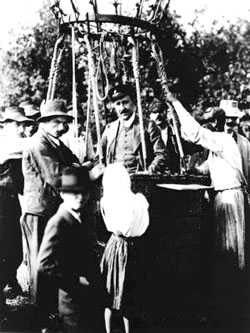
\includegraphics{intro/V-Hess-web_2.jpg}
	\caption{Victor Hess with his famous balloon, 1912.}
\end{marginfigure}

The field of \emph{astroparticle physics}, particle physics with cosmic accelerators, has been a fruitful source of mysteries in recent years. The existence of high-energy charged particles \emph{cosmic rays} was first demonstrated by Victor Hess in 191n, but their origin remains unknown over a century later. In that century, the ghostly neutrino particle was first proposed by Pauli in 192n, its existence was confirmed by in Y, its centrality in solar fusion was first posited by N, the solar neutrino flux was then measured in Z with at an unexpectedly-low rate (the so-called \emph{solar neutrino problem}), which then led to the first discovery of physics outside the Standard Model of particle physics, namely \emph{neutrino oscillations}. Experiments studying these solar neutrinos also accidentally provided us with the first case of observational astronomy with multiple 'messengers' (the observation of nearby supernova SN1987a with both neutrinos and photons), followed by the discovery of extra-terrestrial high-energy \emph{astrophyiscal neutrinos} with the IceCube detector in 2013 produced by the very same cosmic accelerators responsible for cosmic rays. A scramble to find the origin of these neutrinos led to the birth of a new field, \emph{neutrino astronomy}. The long-awaited discovery of Gravitational Waves by LIGO in 2015 was shortly thereafter followed by the discovery of a Binary Neutrino Star merger (GW170817) detected simultaneously with both photons and gravitational waves, kick-starting \emph{gravitational-wave astronomy}. One month later, the observation of a high-energy neutrino IC170922A from the direction of a flaring galactic nucleus led to the identification of the first likely source of high-energy neutrinos, TXS 0506+056. Thirty years after SN1987A, the year 2017 truly marked the dawn of an era of \emph{multi-messenger astronomy}. 


\begin{marginfigure}
	\centering 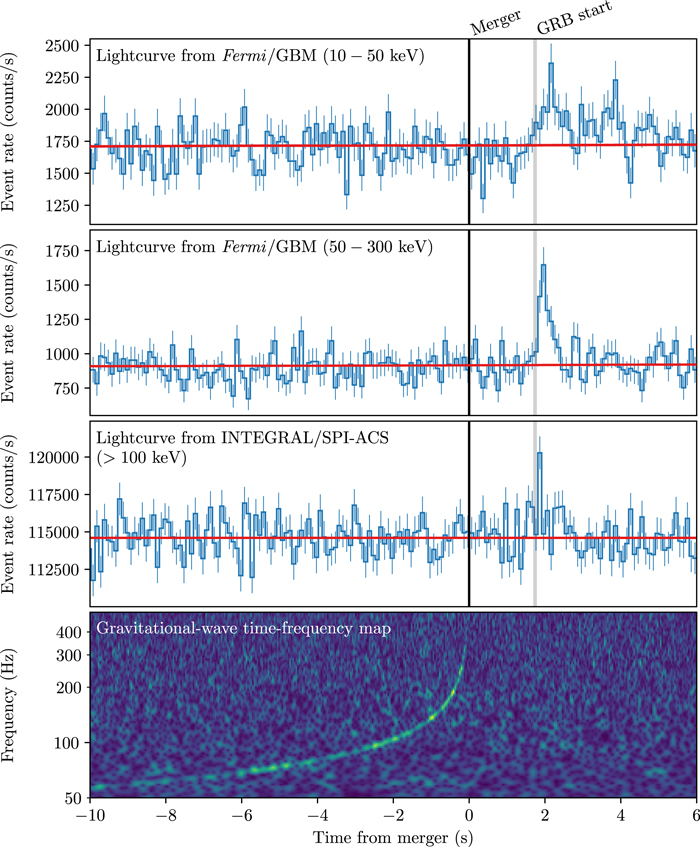
\includegraphics{intro/apjlaa920cf2_lr.jpg}
	\caption{The detection of a binary neutron star merger with photons (upper 3 panels) and gravitational waves (lower panel)  (from CITE).}
\end{marginfigure}

This thesis presents research probing the intersect of these new branches of astronomy with multiple messengers, incorporating searches for sources of neutrinos and gravitational waves using photons, and searches for photon sources using neutrinos. At its core, it seeks to understand what can be learned through combining knowledge from these new branches of astronomy with that of the oldest, namely photon astronomy as observed optical telescopes. The latter field is undergoing a revolution of its own, at the brink of transition from a mature human-driven field characterised by  of to an algorithm-driven one dominated by enormous data volumes. Optical astronomy is moving from object-centric to population-centric science, with scales at which detailed study of individual objects is becoming infeasible. In all three fields, a focus on rapid automated responses seeks to remove human-dependent latency in observational decisions, so-called \emph{realtime astronomy}. This drive was central in the identification of both GW170817 and TXS 0506+056, and forms a central part of this work.

This thesis begins with an introduction to ...





\pagelayout{wide} % No margins
\addpart{Class Options, Commands and Environments}
\pagelayout{margin} % Restore margins

\setchapterpreamble[u]{\margintoc}
\chapter{Class Options}
\labch{options}

In this chapter I will describe the most common options used, both the 
ones inherited from \Class{scrbook} and the \Class{kao}-specific ones. 
Options passed to the class modifies its default behaviour; beware 
though that some options may lead to unexpected results\ldots

\section{\Class{KOMA} Options}

The \Class{kaobook} class is based on \Class{scrbook}, therefore it 
understands all of the options you would normally pass to that class. If 
you have a lot of patience, you can read the \KOMAScript\xspace 
guide.\sidenote{The guide can be downloaded from 
\url{https://ctan.org/pkg/koma-script?lang=en}.} Actually, the reading 
of such guide is suggested as it is very instructive.

Every \KOMAScript\xspace option you pass to the class when you load it 
is automatically activated. In addition, in \Class{kaobook} some options 
have modified default values. For instance, the font size is 9.5pt and 
the paragraphs are separated by space,\sidenote[-7mm][]{To be precise, 
they are separated by half a line worth of space: the \Option{parskip} 
value is \enquote{half}.} not marked by indentation.

\section{\Class{kao} Options}

In the future I plan to add more options to set the paragraph formatting 
(justified or ragged) and the position of the margins (inner or outer in 
twoside mode, left or right in oneside mode).\sidenote{As of now, 
paragraphs are justified, formatted with \Command{singlespacing} (from 
the \Package{setspace} package) and \Command{frenchspacing}.}

I take this opportunity to renew the call for help: everyone is 
encouraged to add features or reimplement existing ones, and to send me 
the results. You can find the GitHub repository at 
\url{https://github.com/fmarotta/kaobook}.

\begin{kaobox}[frametitle=To Do]
Implement the \Option{justified} and \Option{margin} options. To be 
consistent with the \KOMAScript\xspace style, they should accept a 
simple switch as a parameter, where the simple switch should be 
\Option{true} or \Option{false}, or one of the other standard values for 
simple switches supported by \KOMAScript. See the \KOMAScript\xspace 
documentation for further information.
\end{kaobox}

The above box is an example of a \Environment{kaobox}, which will be 
discussed more thoroughly in \frefch{mathematics}. Throughout the book I 
shall use these boxes to remarks what still needs to be done.

\section{Other Things Worth Knowing}

A bunch of packages are already loaded in the class because they are 
needed for the implementation. These include:

\begin{itemize}
	\item etoolbox
	\item calc
	\item xifthen
	\item xkeyval
	\item xparse
	\item xstring
\end{itemize}

Many more packages are loaded, but they will be discussed in due time. 
Here, we will mention only one more set of packages, needed to change 
the paragraph formatting (recall that in the future there will be 
options to change this). In particular, the packages we load are:

\begin{itemize}
	\item ragged2e
	\item setspace
	\item hyphenat
	\item microtype
	\item needspace
	\item xspace
	\item xcolor (with options \Option{usenames,dvipsnames})
\end{itemize}

Some of the above packages do not concern paragraph formatting, but we 
nevertheless grouped them with the others. By default, the main text is 
justified and formatted with singlespacing and frenchspacing; the margin 
text is the same, except that the font is a bit smaller.

\section{Document Structure}

We provide optional arguments to the \Command{title} and 
\Command{author} commands so that you can insert short, plain text 
versions of this fields, which can be used, typically in the half-title 
or somewhere else in the front matter, through the commands 
\Command{@plaintitle} and \Command{@plainauthor}, respectively. The PDF 
properties \Option{pdftitle} and \Option{pdfauthor} are automatically 
set by hyperref to the plain values if present, otherwise to the normal 
values.\sidenote[-1.4cm][]{We think that this is an important point so 
we remark it here. If you compile the document with pdflatex, the PDF 
metadata will be altered so that they match the plain title and author 
you have specified; if you did not specify them, the metadata will be 
set to the normal title and author.}

There are defined two page layouts, \Option{margin} and \Option{wide}, 
and two page styles, \Option{plain} and \Option{fancy}. The layout 
basically concern the width of the margins, while the style refers to 
headers and footer; these issues will be 
discussed in \frefch{layout}.\sidenote{For now, suffice it to say that pages with 
the \Option{margin} layout have wide margins, while with the 
\Option{wide} layout the margins are absent. In \Option{plain} pages the 
headers and footer are suppressed, while in \Option{fancy} pages there 
is a header.} 

The commands \Command{frontmatter}, \Command{mainmatter}, and 
\Command{backmatter} have been redefined in order to automatically 
change page layout and style for these sections of the book. The front 
matter uses the \Option{margin} layout and the \Option{plain} page 
style. In the mainmatter the margins are wide and the headings are 
fancy. In the appendix the style and the layout do not change; however 
we use \Command{bookmarksetup\{startatroot\}} so that the bookmarks of 
the chapters are on the root level (without this, they would be under 
the preceding part). In the backmatter the margins shrink again and we 
also reset the bookmarks root.

\setchapterpreamble[u]{\margintoc}
\chapter{Margin Stuff}

Sidenotes are a distinctive feature of all 1.5-column-layout books. 
Indeed, having wide margins means that some material can be displayed 
there. We use margins for all kind of stuff: sidenotes, marginnotes, 
small tables of contents, citations, and, why not?, special boxes and 
environments.

\section{Sidenotes}

Sidenotes are like footnotes, except that they go in the margin, where 
they are more readable. To insert a sidenote, just use the command 
\Command{sidenote\{Text of the note\}}. You can specify a 
mark\sidenote[O]{This sidenote has a special mark, a big O!} with \\ 
\Command{sidenote[mark]\{Text\}}, but you can also specify an offset, 
which moves the sidenote upwards or downwards, so that the full syntax is:

\begin{lstlisting}[style=kaolstplain]
\sidenote[offset][mark]{Text}
\end{lstlisting}

If you use an offset, you always have to add the 
brackets for the mark, but they can be empty.\sidenote{If you want to 
know more about the usage of the \Command{sidenote} command, read the 
documentation of the \Package{snotez} package.} The format of the actual 
sidenote can be changed with the command \Command{setsidenotes}, which 
allows you to modify, for instance, the format of the markers and the 
separator between the marker and the text of the sidenote.

There was an alternative package, \Package{sidenotes}, which we could 
have used. In the end we went for \Package{snotez} because it was the 
one used in Ken Ohori's thesis, which inspired this class. The features 
are very similar, but one additional thing offered by \Package{snotez} 
is that the offset can be specified as a multiple of 
\Command{baselineskip}. For example, if you want to enter a sidenote 
with the normal mark and move it upwards one line, type:

\begin{lstlisting}[style=kaolstplain]
\sidenote[*-1][]{Text of the sidenote.}
\end{lstlisting}

Sidenotes are handled through the \Package{snotez} package, which in 
turn relies on the \Package{marginnote} package.

\section{Marginnotes}

This command is very similar to the previous one. You can create a 
marginnote with \Command{marginnote[offset]\{Text\}}, where the offset 
argument can be left out, or it can be a multiple of 
\Command{baselineskip},\marginnote[-1cm]{While the command for margin 
notes comes from the \Package{marginnote} package, it has been redefined 
in order to change the position of the optional offset argument, which 
now precedes the text of the note, whereas in the original version it 
was at the end. We have also added the possibility to use a multiple of 
\Command{baselineskip} as offset. These things were made only to make 
everything more consistent, so that you have to remember less things!} 
\eg

\begin{lstlisting}[style=kaolstplain]
\marginnote[-12pt]{Text} or \marginnote[*-3]{Text}
\end{lstlisting}

\begin{kaobox}[frametitle=To Do]
A small thing that needs to be done is to renew the \Command{sidenote} 
command so that it takes only one optional argument, the offset. The 
special mark argument can go somewhere else. In other words, we want the 
syntax of \Command{sidenote} to resemble that of \Command{marginnote}.
\end{kaobox}

We load the packages \Package{marginnote}, \Package{marginfix} and 
\Package{placeins}. Since \Package{snotez} uses \Package{marginnote}, 
what we said for marginnotes is also valid for sidenotes. Side- and 
margin- notes are shifted slightly upwards 
(\Command{renewcommand\{\textbackslash marginnotevadjust\}\{3pt\}}) in 
order to allineate them to the bottom of the line of text where the note 
is issued.

\section{Footnotes}

Even though they are not displayed in the margin, we will discuss about 
footnotes here, since sidenotes are mainly intended to be a replacement 
of them. Footnotes force the reader to constantly move from one area of 
the page to the other. Arguably, marginnotes solve this issue, so you 
should not use footnotes. Nevertheless, for completeness, we have left 
the standard command \Command{footnote}, just in case you want to put a 
footnote once in a while.\footnote{And this is how they look like. 
Notice that in the PDF file there is a back reference to the text; 
pretty cool, uh?}

\section{Margintoc}

Since we are talking about margins, we introduce here the 
\Command{margintoc} command, which allows one to put small table of 
contents in the margin. Like other commands we have discussed, 
\Command{margintoc} accepts a parameter for the vertical offset, like 
so: \Command{margintoc[offset]}.

The command can be used in any point of the document, but we think it 
makes sense to use it just at the beginning of chapters or parts. In 
this document I make use of a \KOMAScript\xspace feature and put it in 
the chapter preamble, with the following code:

\marginnote{The font used in the margintoc is the same as the one for 
	the chapter entries in the main table of contents at the beginning 
	of the document.}

\begin{lstlisting}[style=kaolstplain]
\setchapterpreamble[u]{\margintoc}
\chapter{Chapter title}
\end{lstlisting}

Not only textual stuff can be displayed in the margin, but also figures. 
Those will be the focus of the next chapter.

\setchapterimage[6.5cm]{seaside}
\setchapterpreamble[u]{\margintoc}
\chapter[Figures and Tables]{Figures and Tables\footnotemark[0]}

\footnotetext{The credits for the image above the chapter title go to:
	Bushra Feroz --- Own work, CC~BY-SA~4.0, 
	\url{https://commons.wikimedia.org/w/index.php?curid=68724647}}

\section{Normal Figures and Tables}

Figures and tables can be inserted just like in any standard 
\LaTeX\xspace document. The \Package{graphicx} package is already loaded 
and configured in such a way that the figure width is equal to the 
textwidth and the height is adjusted in order to maintaini the original 
aspect ratio. As you may have imagined, the captions will be 
positioned\ldots well, in the margins. This is achieved with the help of 
the \Package{floatrow} package.

Here is a picture of Mona Lisa (\reffig{normalmonalisa}), as an example. 
The captions are formatted as the margin- and the side-notes; If you 
want to change something about captions you can use the command 
\Command{captsetup} from the \Package{caption} package. Remember that if 
you want to reference a figure, the label must come \emph{after} the 
caption!

\begin{figure}[hb]
	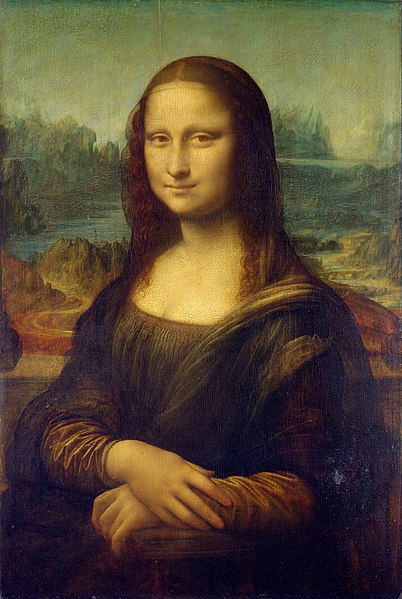
\includegraphics[width=0.45\textwidth]{monalisa}
	\caption[Mona Lisa, again]{It's Mona Lisa again. \blindtext}
	\labfig{normalmonalisa}
\end{figure}

While the format of the caption is managed by \Package{caption}, its 
position is handled by the \Package{floatrow} package. Achieving this 
result has been quite hard, but now I am pretty satisfied. In two-side 
mode, the captions are printed in the correct margin.

Tables can be inserted just as easily as figures, as exemplified by the 
following code:

\begin{lstlisting}
\begin{table}
\begin{tabular}{ c c c c }
	\toprule
	col1 & col2 & col3 & col 4 \\
	\midrule
	\multirow{3}{4em}{Multiple row} & cell2 & cell3 & cell4\\ &
	cell5 & cell6 & cell7 \\ &
	cell8 & cell9 & cell10 \\
	\multirow{3}{4em}{Multiple row} & cell2 & cell3 & cell4 \\ &
	cell5 & cell6 & cell7 \\ &
	cell8 & cell9 & cell10 \\
	\bottomrule
\end{tabular}
\end{table}
\end{lstlisting}

which results in the useless \vreftab{useless}.

\begin{table}[h]
\caption[A useless table]{A useless table.}
\labtab{useless}
\begin{tabular}{ c c c c }
	\toprule
	col1 & col2 & col3 & col 4 \\
	\midrule
	\multirow{3}{4em}{Multiple row} & cell2 & cell3 & cell4\\ &
	cell5 & cell6 & cell7 \\ &
	cell8 & cell9 & cell10 \\
	\multirow{3}{4em}{Multiple row} & cell2 & cell3 & cell4 \\ &
	cell5 & cell6 & cell7 \\ &
	cell8 & cell9 & cell10 \\
	\bottomrule
\end{tabular}
\end{table}

I don't have much else to say, so I will just insert some blind text. 
\blindtext

\section{Margin Figures and Tables}

Marginfigures can be inserted with the environment 
\Environment{marginfigure}. In this case, the whole picture is confined 
to the margin and the caption is below it. \reffig{marginmonalisa} is 
obtained with something like this:

\begin{lstlisting}
\begin{marginfigure}
	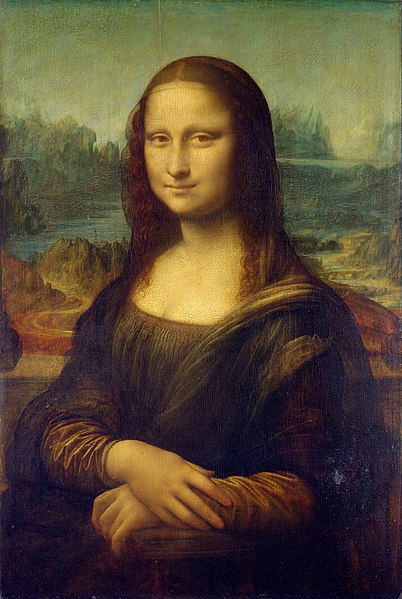
\includegraphics{monalisa}
	\caption[The Mona Lisa]{The Mona Lisa.}
	\labfig{marginmonalisa}
\end{marginfigure}
\end{lstlisting}

There is also the \Environment{margintable} environment, of which 
\reftab{anotheruseless} is an example. Notice how you can place the 
caption above the table by just placing the \Command{caption} command 
before beginning the \Environment{tabular} environment. Usually, figure 
captions are below, while table captions are above. This rule is also 
respected for normal figures and tables: the captions are always on the 
side, but for figure they are aligned to the bottom, while for tables to 
the top.

\begin{margintable}
\caption[Another useless table]{Another useless table.}
\labtab{anotheruseless}
\raggedright
\begin{tabular}{ c c c c }
	\hline
	col1 & col2 & col3 \\
	\hline
	\multirow{3}{4em}{Multiple row} & cell2 & cell3 \\ & cell5 & cell6 
	\\ & cell8 & cell9 \\ \hline
\end{tabular}
\end{margintable}

Marginfigures and tables can be positioned with an optional offset 
command, like so:

\begin{lstlisting}
\begin{marginfigure}[offset]
	\includegraphics{images/seaside}
\end{marginfigure}
\end{lstlisting}

Offset ca be either a measure or a multiple of \Command{baselineskip}, 
much like with \Command{sidenote}, \Command{marginnote} and 
\Command{margintoc}.\todo{Improve this part.} If you are wondering how I 
inserted this orange bubble, have a look at the \Package{todo} package.

\section{Wide Figures and Tables}

\begin{figure*}[h!]
	\includegraphics{seaside}
	\caption[A wide seaside]{A wide seaside, and a wide caption.
		Credits: By Bushra Feroz --- Own work, CC BY-SA 4.0, 
		\url{https://commons.wikimedia.org/w/index.php?curid=68724647}}
\end{figure*}

With the environments \Environment{figure*} and \Environment{table*} you 
can insert figures which span the whole page width. The caption will be 
positioned below or above, according to taste.

You may have noticed the full width image at the very beginning of this 
chapter: that, however, is set up in an entirely different way, which 
you'll read about in \vrefch{layout}. Now it is time to tackle 
hyperreferences.

\setchapterstyle{kao}
%\setchapterpreamble[u]{\margintoc}
\chapter{References}
\labch{references}

\section{Citations}

\index{citations}
To cite someone \sidecite{Visscher2008,James2013} is very simple: just 
use the \Command{sidecite}\index{\Command{sidecite}} command. It does 
not have an offset argument yet, but it probably will in the future. 
This command supports multiple entries, as you can see, and by default 
it prints the reference on the margin as well as adding it to the 
bibliography at the end of the document. For this setup I used biblatex 
but I think that workarounds are possible.\sidecite{James2013} Note that 
the citations have nothing to do with the text, they are completely 
random as they only serve the purpose to illustrate the feature.

To compile a document containing citations, you need to use an external 
tool, which for this class is biber. You need to run the following 
(assuming that your tex file is called main.text):

\begin{lstlisting}[style=kaolstplain]
$ pdflatex main
$ biber main
$ pdflatex main
\end{lstlisting}

\section{Glossaries and Indices}

\index{glossary}
The \Class{kaobook} class loads the packages \Package{glossaries} and 
\Package{imakeidx}, with which you can add glossaries and indices to 
your book. For instance, I previously defined some glossary entries and 
now I am going to use them, like this: \gls{computer}. 
\Package{glossaries} also allows you to use acronyms, like the 
following: this is the full version, \acrfull{fpsLabel}, and this is the 
short one \acrshort{fpsLabel}. These entries will appear in the glossary 
in the backmatter.

Unless you use \href{https://www.overleaf.com}{Overleaf} or some other 
fancy IDE for \LaTeX, you need to run an external command from your 
terminal in order to compile a document with a glossary. In particular, 
the commands required are:\sidenote[-2mm][]{These are the commands you 
would run in a UNIX system; I have no idea on how it works in Windows.}

\begin{lstlisting}[style=kaolstplain]
$ pdflatex main
$ makeglossaries main
$ pdflatex main
\end{lstlisting}

Note that you need not run \texttt{makeglossaries} every time you 
compile your document, but only when you change the glossary entries.

\index{index}
To create an index, you need to insert the command 
\lstinline|\index{subject}| whenever you are talking about 
\enquote{subject} in the text. For instance, at the start of this 
paragraph I would write \lstinline|index{index}|, and an entry would be 
added to the Index in the backmatter. Check it out!

\marginnote[2mm]{In theory, you would need to run an external command 
for the index as well, but luckily the package we suggested, 
	\Package{imakeidx}, can compile the index automatically.}

\index{nomenclature}
A nomenclature is just a special kind of index; you can find one at the end of
this book. To insert a nomenclature, we use the package \Package{nomencl} and
add the terms with the command \Command{nomenclature}. We put then a
\Command{printnomenclature} where we want it to appear.

Also with this package we need to run an external command to compile the 
document, otherwise the nomenclature will not appear:

\begin{lstlisting}[style=kaolstplain]
$ pdflatex main
$ makeindex main.nlo -s nomencl.ist -o main.nls
$ pdflatex main
\end{lstlisting}

These packages are all loaded in 
\href{style/packages.sty}{packages.sty}, one of the files that come with 
this class. However, the configuration of the elements is best done in 
the main.tex file, since each book will have different entries and 
styles.

Note that the \Package{nomencl} package caused problems when the 
document was compiled, so, to make a long story short, I had to prevent 
\Package{scrhack} to load the hack-file for \Package{nomencl}. When 
compiling the document on Overleaf, however, this problem seem to 
vanish.

\marginnote[-19mm]{This brief section was by no means a complete 
reference on the subject, therefore you should consult the documentation 
of the above package to gain a full understanding of how they work.}

\section{Hyperreferences}

\index{hyperreferences}
In this class we provide a handy sub-package to help you referencing the 
same elements always in the same way, for consistency across the book. 
First, you can label each element with a specific command. For instance, 
should you want to label a chapter, you would put 
\lstinline|\labch{chapter-title}| right after the \Command{chapter} 
directive. This is just a convienence, because \Command{labch} is 
actually just an alias to \lstinline|\label{ch:chapter-title}|, so it 
spares you the writing of \enquote{ch}. We defined similar commands for 
many typically labeled elements, including:

\begin{multicols}{2}
\setlength{\columnseprule}{0pt}
\begin{itemize}
	\item Page: \Command{labpage}
	\item Part: \Command{labpart}
	\item Chapter: \Command{labch}
	\item Section: \Command{labsec}
	\item Figure: \Command{labfig}
	\item Table: \Command{labtab}
	\item Definition: \Command{labdef}
	\item Theorem: \Command{labthm}
	\item Proposition: \Command{labprop}
	\item Lemma: \Command{lablemma}
	\item Remark: \Command{labremark}
	\item Example: \Command{labexample}
	\item Exercise: \Command{labexercise}
\end{itemize}
\end{multicols}

Of course, we have similar commands for referencing those elements. 
However, since the style of the reference should depend on the context, 
we provide different commands to reference the same thing. For instance, 
in some occasions you may want to reference the chapter by name, but 
other times you want to reference it only by number. In general, there 
are four reference style, which we call plain, vario, name, and full. 

The plain style references only by number. It is accessed, for chapters, 
with \lstinline|\refch{chapter-title}| (for other elements, the syntax 
is analogous). Such a reference results in: \refch{references}.

The vario and name styles rest upon the \Package{varioref} package. 
Their syntax is \lstinline|\vrefch{chapter-title}| and 
\lstinline|\nrefch{chapter-title}|, and they result in: 
\vrefch{references}, for the vario style, and: \nrefch{references}, for 
the name style. As you can see, the page is referenced in 
\Package{varioref} style.

The full style references everything. You can use it with 
\lstinline|\frefch{chapter-title}| and it looks like this: 
\frefch{references}.

Of course, all the other elements have similar commands (\eg for parts 
you would use \lstinline|\vrefpart{part-title}| or something like that). 
However, not all elements implement all the four styles. The commands 
provided should be enough, but if you want to see what is available or 
to add the missing ones, have a look at the 
\href{styles/references.sty}{attached package}.


\pagelayout{wide} % No margins
\addpart{Design and Additional Features}
\pagelayout{margin} % Restore margins

\setchapterimage[6cm]{images/seaside}
\setchapterpreamble[u]{\margintoc}
\chapter{Page Design}
\labch{layout}

\section{Headings}

So far, in this document I used two different styles for the chapter 
headings: one has the chapter name, a rule and, in the margin, the 
chapter number; the other has an image at the top of the page, and the 
chapter title is printed in a box (like for this chapter). There is one 
additional style, which I used only in the appendix 
(\vrefpage{appendix}); there, the chapter title is enclosed in two 
horizontal rules, and the chapter number (or letter, in the case of the 
appendix) is above it.\sidenote{To be honest, I do not think that mixing 
heading styles like this is a wise choice, but in this document I did 
only to show you how they look.}

Every book is unique, so it makes sense to have different styles from 
which to choose. Actually, it would be awesome if whenever a 
\Class{kao}-user designs a new heading style, he or she added it to the 
three styles already present, so that it will be available for new users 
and new books.

The choice of the style is made simple by the \Command{setchapterstyle} 
command. It accepts one option, the name of the style, which can be: 
\enquote{plain}, \enquote{kao}, or \enquote{lines}.\sidenote{Plain is 
the default \LaTeX\xspace title style; the other ones are self 
explanatory.} If instead you want the image style, you have to use the 
command \Command{setchapterimage}, which accepts the path to the image 
as argument; you can also provide an optional parameter in square 
brackets to specify the height of the image.

Let us make some examples. In this book, I begin a normal chapter with 
the lines:

\begin{lstlisting}
\setchapterstyle{kao}
\setchapterpreamble[u]{\margintoc}
\chapter{Title of the Chapter}
\labch{title}
\end{lstlisting}

In Line 1 I choose the style for the title to be \enquote{kao}. Then, I 
specify that I want the margin toc. The rest is ordinary administration 
in \LaTeX, except that I use my own \Command{labch} to label the 
chapter. Actually, the \Command{setchapterpreamble} is a standard 
\KOMAScript\xspace one, so I invide you to read about it in the KOMA 
documentation. Once the chapter style is set, it holds until you change 
it.\sidenote{The \Command{margintoc} has to be specified at every 
chapter. Perhaps in the future this may change; it all depends on how 
this feature will be welcomed by the users, so keep in touch with me if 
you have preferences!} Whenever I want to start a chapter with an image, 
I simply write:

\begin{lstlisting}
\setchapterimage[7cm]{path/to/image.png} % Optionally specify the height
\setchapterpreamble[u]{\margintoc}
\chapter{Catchy Title} % No need to set a chapter style
\labch{catchy}
\end{lstlisting}

\section{Headers \& Footers}

Headers and footers in \KOMAScript\xspace are handled by the 
\Package{scrlayer-scrpage} package. There are two basic style: 
\enquote{scrheadings} and \enquote{plain.scrheadings}. The former is 
used for normal pages, whereas the latter is used in title pages (those 
where a new chapter starts, for instance) and, at least in this book, in 
the front matter. At any rate, the style can be changed with the 
\Command{pagestyle} command, \eg 
\lstinline|\pagestyle{plain.scrheadings}|.

In both stles, the footer is completely empty. In plain.scrheadings, 
also the header is absent (otherwise it wouldn't be so plain\ldots), but 
in the normal style the design is reminescent of the \enquote{kao} style 
for chapter titles.

\begin{kaobox}[frametitle=To Do]
The \Option{twoside} class option is still unstable and. As always, any 
help will be greatly appreciated.
\end{kaobox}

\section{Table of Contents}

Another important part of a book is the table of contents. By default, 
in \Class{kaobook} there is an entry for everything: list of figures, 
list of tables, bibliographies, and even the table of contents itself. 
Not everybody might like this, so we will provide a description of the 
changes you need to do in order to enable or disable each of these 
entries. In the following \reftab{tocentries}, each item corresponds to 
a possible entry in the \acrshort{tocLabel}, and its description is the 
command you need to provide to have such entry. These commands are 
specified in the attached \href{style/style.sty}{style 
package},\sidenote{In the same file, you can also choose the titles of 
these entries.} so if you don't want the entries, just comment the 
corresponding lines.

Of course, some packages, like those for glossaries and indices, will 
try to add their own entries.\marginnote{In a later section, we will see 
how you can define your own floating environment, and endow it with an 
entry in the \acrshort{tocLabel}.} In such cases, you have to follow the 
instructions specific to that package. Here, since we have talked about 
glossaries and notations in \refch{references}, we will biefly see how 
to configure them.

\begin{table}
\footnotesize
\caption{Commands to add a particular entry to the table of contents.}
\labtab{tocentries}
\begin{tabular}{ l l }
	\toprule
	Entry & Command to Activate \\
	\midrule
	Table of Contents & \lstinline|\setuptoc{toc}{totoc}| \\
	List of Figs and Tabs & \lstinline|\PassOptionsToClass{toc=listof}{\@baseclass}| \\
	Bibliography & \lstinline|\PassOptionsToClass{toc=bibliography}{\@baseclass}| \\
	\bottomrule
\end{tabular}
\end{table}

For the \Package{glossaries} package, use the \enquote{toc} option when 
you load it: \lstinline|\usepackage[toc]{glossaries}|. For 
\Package{nomencl}, pass the \enquote{intoc} option at the moment of 
loading the package. Both \Package{glossaries} and \Package{nomencl} are 
loaded in the attached \href{style/packages.sty}{\enquote{packages} 
package}.

Additional configuration of the table of contents can be performed 
through the packages \Package{etoc}, which is loaded because it is 
needed for the margintocs, or the more traditional \Package{tocbase}. 
Read the respective documentations if you want to be able to change the 
default \acrshort{tocLabel} style.\sidenote{(And please, send me a copy 
of what you have done, I'm so curious!)}

\section{Page Layout}

Besides the page style, you can also change the width of the content of 
a page. This is particularly useful for pages dedicated to part titles, 
where having the 1.5-column layout might be a little awkward, or for 
pages where you only put figures, where it is important to exploit all 
the available space.

In practice, there are two layouts: \enquote{wide} and \enquote{margin}. 
The former suppresses the margins and allocates the full page for 
contents, while the latter is the layout used in most of the pages of 
this book, including this one. The wide layout is also used 
automatically in the front and back matters.

To change page layout, use the \Command{pagelayout} command. For 
example, when I start a new part, I write:

\begin{lstlisting}
\pagelayout{wide}
\addpart{Title of the New Part}
\pagelayout{margin}
\end{lstlisting}

\section{Numbers \& Counters}

In this short section we shall see how dispositions, sidenotes and 
figures are numbered in the \Class{kaobook} class.

By default, dispositions are numbered up to the section. This is 
achieved by setting: \lstinline|\setcounter{secnumdepth}{1}|.

The sidenotes counter is the same across all the document, but if you 
want it to reset at each chapter, just uncomment the line

\begin{lstlisting}[style=kaolstplain]
\counterwithin*{sidenote}{chapter}
\end{lstlisting}

in the \Package{styles/style.sty} package provided by this class.

Figure and Table numbering is also per-chapter; to change that, use 
something like:

\begin{lstlisting}[style=kaolstplain]
\renewcommand{\thefigure}{\arabic{section}.\arabic{figure}}
\end{lstlisting}

\section{White Space}

One of the things that I find most hard in \LaTeX\xspace is to finely 
tune the white space around objects. There are not fixed rules, each 
object needs its own adjustment. Here we shall see how some spaces are 
defined at the moment in this class.\marginnote{Attention! This section 
may be incomplete.}

\textbf{Space around figures and tables}

\begin{lstlisting}[style=kaolstplain]
\renewcommand\FBaskip{.4\topskip}
\renewcommand\FBbskip{\FBaskip}
\end{lstlisting}

\textbf{Space around captions}

\begin{lstlisting}[style=kaolstplain]
\captionsetup{
	aboveskip=6pt,
	belowskip=6pt
}
\end{lstlisting}

\textbf{Space around displays (\eg equations)}

\begin{lstlisting}[style=kaolstplain]
\setlength\abovedisplayskip{6pt plus 2pt minus 4pt}
\setlength\belowdisplayskip{6pt plus 2pt minus 4pt}
\abovedisplayskip 10\p@ \@plus2\p@ \@minus5\p@
\abovedisplayshortskip \z@ \@plus3\p@
\belowdisplayskip \abovedisplayskip
\belowdisplayshortskip 6\p@ \@plus3\p@ \@minus3\p@
\end{lstlisting}

\setchapterstyle{kao}
\setchapterpreamble[u]{\margintoc}
\chapter{Mathematics and Boxes}
\labch{mathematics}

\section{Theorems}

Despite most people complain at the sight of a book full of equations, 
mathematics is an important part of many books. Here, we shall 
illustrate some of the possibilities. We believe that theorems, 
definitions, remarks and examples should be emphasised with a shaded 
background; however, the colour should not be to heavy on the eyes, so 
we have chosen a sort of light yellow.\sidenote{The boxes are all of the 
same colour here, because we did not want our document to look like 
\href{https://en.wikipedia.org/wiki/Harlequin}{Harlequin}.}

\begin{definition}
\labdef{openset}
Let $(X, d)$ be a metric space. A subset $U \subset X$ is an open set 
if, for any $x \in U$ there exists $r > 0$ such that $B(x, r) \subset 
U$. We call the topology associated to d the set $\tau\textsubscript{d}$ 
of all the open subsets of $(X, d).$
\end{definition}

\refdef{openset} is very important. I am not joking, but I have inserted 
this phrase only to show how to reference definitions. The following 
statement is repeated over and over in different environments.

\begin{theorem}
A finite intersection of open sets of (X, d) is an open set of (X, d), 
i.e $\tau\textsubscript{d}$ is closed under finite intersections. Any 
union of open sets of (X, d) is an open set of (X, d).
\end{theorem}

\begin{proposition}
A finite intersection of open sets of (X, d) is an open set of (X, d), 
i.e $\tau\textsubscript{d}$ is closed under finite intersections. Any 
union of open sets of (X, d) is an open set of (X, d).\marginnote{You can even insert footnotes inside the theorem 
	environments; they will be displayed at the bottom of the box.}
\end{proposition}

\begin{lemma}
A finite intersection\footnote{I'm a footnote} of open sets of (X, d) is 
an open set of (X, d), i.e $\tau\textsubscript{d}$ is closed under 
finite intersections. Any union of open sets of (X, d) is an open set of 
(X, d).
\end{lemma}

You can safely ignore the content of the theorems\ldots I assume that if 
you are interested in having theorems in your book, you already know 
something about the classical way to add them. These example should just 
showcase all the things you can do within this class.

\begin{corollary}[Finite Intersection, Countable Union]
A finite intersection of open sets of (X, d) is an open set of (X, d), 
i.e $\tau\textsubscript{d}$ is closed under finite intersections. Any 
union of open sets of (X, d) is an open set of (X, d).
\end{corollary}

\begin{proof}
The proof is left to the reader as a trivial exercise. Hint: \blindtext
\end{proof}

\begin{definition}
Let $(X, d)$ be a metric space. A subset $U \subset X$ is an open set 
if, for any $x \in U$ there exists $r > 0$ such that $B(x, r) \subset 
U$. We call the topology associated to d the set $\tau\textsubscript{d}$ 
of all the open subsets of $(X, d).$\marginnote{
	Here is a random equation, just because we can:
	\begin{equation*}
  x = a_0 + \cfrac{1}{a_1
          + \cfrac{1}{a_2
          + \cfrac{1}{a_3 + \cfrac{1}{a_4} } } }
	\end{equation*}
}
\end{definition}

\begin{example}
Let $(X, d)$ be a metric space. A subset $U \subset X$ is an open set 
if, for any $x \in U$ there exists $r > 0$ such that $B(x, r) \subset 
U$. We call the topology associated to d the set $\tau\textsubscript{d}$ 
of all the open subsets of $(X, d).$
\end{example}

\begin{remark}
Let $(X, d)$ be a metric space. A subset $U \subset X$ is an open set 
if, for any $x \in U$ there exists $r > 0$ such that $B(x, r) \subset 
U$. We call the topology associated to d the set $\tau\textsubscript{d}$ 
of all the open subsets of $(X, d).$
\end{remark}

As you may have noticed, definitions, example and remarks have 
independent counters; theorems, propositions, lemmas and corollaries 
share the same counter.

\begin{remark}
Here is how an integral looks like inline: $\int_{a}^{b} x^2 dx$, and 
here is the same integral displayed in its own paragraph:
\[\int_{a}^{b} x^2 dx\]
\end{remark}

We provide two files for the theorem styles: 
\href{style/plaintheorems.sty}{plaintheorems.sty}, which you should 
include if you do not want coloured boxes around theorems; and 
\href{style/mdftheorems.sty}{mdftheorems.sty}, which is the one used for 
this document.\sidenote{The plain one is not showed, but actually it is 
exactly the same as this one, only without the yellow boxes.} Of course, 
you will have to edit these files according to your taste and the 
general style of the book.

\section[Boxes \& Environments]{Boxes \& Custom Environments
\sidenote[*1.6][]{Notice that in the table of contents and in the 
	header, the name of this section is \enquote{Boxes \& Environments}; 
	we achieved this with the optional argument of the \texttt{section} 
	command.}}

Say you want to insert a special section, an optional content or just 
something you want to emphasise. We think that nothing works better than 
a box in these cases. We used \Package{mdframed} to construct the ones 
shown below. You can create and modify such environments by editing the 
provided file \href{style/environments.sty}{environments.sty}.

\begin{kaobox}[frametitle=Title of the box]
\blindtext
\end{kaobox}

If you set up a counter, you can even create your own numbered 
environment.

\begin{kaocounter}
	\blindtext
\end{kaocounter}

\section{Experiments}

It is possible to wrap marginnotes inside boxes, too. Audacious readers 
are encouraged to try their own experiments and let me know the 
outcomes.

\marginnote[-2.2cm]{
	\begin{kaobox}[frametitle=title of margin note]
		Margin note inside a kaobox.\\
		(Actually, kaobox inside a marginnote!)
	\end{kaobox}
}

I believe that many other special things are possible with the 
\Class{kaobook} class. During its development, I struggled to keep it as 
flexible as possible, so that new features could be added without too 
great an effort. Therefore, I hope that you can find the optimal way to 
express yourselves in writing a book, report or thesis with this class, 
and I am eager to see the outcomes of any experiment that you may try.

%\begin{margintable}
	%\captionsetup{type=table,position=above}
	%\begin{kaobox}
		%\caption{caption}
		%\begin{tabular}{ |c|c|c|c| }
			%\hline
			%col1 & col2 & col3 \\
			%\hline
			%\multirow{3}{4em}{Multiple row} & cell2 & cell3 \\ & cell5 
			%%& cell6 \\ 
			%& cell8 & cell9 \\
			%\hline
		%\end{tabular}
	%\end{kaobox}
%\end{margintable}


\setchapterimage[6.5cm]{icecube}
\setchapterpreamble[u]{\margintoc}
\chapter{IceCube Neutrino Observatory}
\labch{icecube}
\begin{fquote}[Edmund Hillary][][1957] I am hell-bent for the South Pole — God willing and crevasses permitting.
\end{fquote}
The IceCube Neutrino Observatory is the world's largest neutrino telescope, located at the geographic south pole. It was built as a successor to the AMANDA experiment, which had pioneered the detection of neutrinos in ice. AMANDA served as a proof of concept for the detection of neutrinos, but with a volume of just nkm$^{3}$, it only had sufficient effective area to measure atmospheric neutrinos. 

IceCube, on the other hand, was envisioned as a much larger detector capable of measuring astrophysical neutrinos. It was constructed in phases from 2006 to 2011, eventually reaching a total volume of one cubic kilometer. 

\section{The IceCube Detector}

IceCube is composed of 86 strings arranged in a hexagonal grid. Each string is 2.5 km long, and carries regularly-spaced Digital Optical Modules (DOMs) containing Photo-Multiplier Tubes (PMTs). With a hot-water drill, holes were drilled into the glacier ice to a depth of 2.5 km. After string deployment, the liquid-filled holes refroze, fixing the DOMs in place. In total, there are 5160 DOMs deployed in IceCube, all at depths greater than 1km. The Antartic ice itself thus provides the detection medium for neutrinos, with the Earth acting as a shield against atmospheric muons.

The design of IceCube is an optimisation trading DOM-density against effective area for fixed cost. A minimal DOM density is needed to identify and reconstruct an event, and this threshold decreases as neutrino energy increases. Thus, while IceCube is generally optimised for detecting high-energy neutrinos in the astrophysical regime, it is far too sparse to effectively measure lower-energy (1-100 GeV) neutrinos. However, in addition to the regular grid of strings, IceCube contains a denser in-fill array known as \textit{Deepcore}. This array consists of 7 strings and n DOMs, and typically uses the outer IceCube detector as a veto against muons?. \textit{Deepcore} measures low-energy neutrinos which form the basis of neutrino oscillation studies, but can also be used for neutrino astronomy at lower energy scales.

IceCube also contains a surface array of instrumented ice tanks known as IceTop, which are used to measure surface air showers arising from cosmic rays and photon interactions. IceTop can be used as a veto against muons from air showers, but only for a small fraction of events which are almost-vertically down-going. However, IceTop also functions in its own right as a Cosmic-Ray detector, and contributes competitive measurements of the cosmic ray flux and composition.

While most event selections for GeV and TeV-PeV neutrinos require multiple DOM hits to reject thermal-noise background, a separate detection channel exists for MeV neutrinos that are typically produced in both stellar fusion and supernova collapse. These neutrinos form an irreducible background for the IceCbe detector, with extremely short track lengths that are only detectable by single DOMs. A dedicated SuperNova Data Aquistion System (SNDAQ) is installed to measure the rate of these single-DOM detections, and identify any significant deviation from expected rates. As demonstrated by SN1987a, any nearby supernova will produce a significant flux of MeV neutrinos during core collapse, and this will be manifested in a significant uptick in trigger rate that will evolve as a function of time. It is predicted that IceCube will be able to clearly measure the temporal evolution of MeV neutrinos from any supernova in the galaxy or Magellanic Clouds, similar to Figure NNNN. IceCube sends any mid-significance deviations from trigger rate to the SuperNova Early Warning System (SNEWS), where they are cross-correlated with other sensitive neutrino detectors such as SNO and Super-K. In the event of a multi-detector trigger, observatories around the world will be alerted to the upcoming optical counterpart of a galactic supernova, which can be localised in the case of a strong signal by combining directional information from individual detectors and time-delays between detectors in differing geographical locations. 



MeV neutrinos for supernovae.

\section{Proposed Improvements to the IceCube detector}

There are several planned or proposed extensions to IceCube that would substantially improve the detector performance. Beginning in 2023, deployment will start for the IceCube Upgrade, a Deepcore-like dense infill array. The string spacing will be even tigher than deepcore, with a higher density of DOMs. In combination with hardware improvements from multi-PMT DOMs, the Upgrade should push IceCube's lower energy threshold from a few GeV, and potentially to below one GeV. This opens up an entirely new regime for both oscillation studies and lower-energy neutrino astronomy relative to competitor neutrino detectors such as SuperK. In addition to the gains from DOMs, many new calibration devices will be deployed to more accurately constrain sources of systematic uncertainties, in particular the ice scattering and absorption length. With these calibration measurements, archival neutrino data can be reprocessed, providing more accurate reconstructed parameters. Improvement should be expected for all neutrino sources analyses, which all suffer to lesser or greater degree from these systematic errors. 

Beyond the IceCube Upgrade, a more comprehensive improvement is planned to extend the higher-energy capability of IceCube. IceCube-Gen2 is a proposed extension instrumenting 10 km$^{3}$ of ice, with a sparser string footprint than the existing detector. While multi-PMT DOMs should partially compensate the lower density, Gen2 represents a transition in focus to higher-energy neutrinos at 10TeV-100PeV range, at the cost of poorer resolution for lower-energy neutrinos with few DOM hits. Given the tenfold increase in instrumented volume, IceCube Gen2 will substantially increase sensitivity to both steady and time-dependent neutrino sources.

A further radio-based extension is proposed to complement the DOM-based Gen2 component. The detection of radio-based air shower detection has been demonstrated by the Pierre Auger Observatory, and its use in ice was pioneered by the ARA and ARIANNA collaborations. A pilot array for neutrino detection is currently being depolyed in Greenland. Radio-based observatories are cheap, and given the possibility of single-station shower detection, an extremely sparse array can be deployed to substantially boost effective area. The proposed radio-based component for Gen2, covering n000 stations, would significantly improve sensitivity at the higher energies beyond nPeV, and could additionally probe the cosmogenic neutrino flux produced by interactions of UHECRs and CMB photons.

IceAct?

\section{Detecting interactions in IceCube}

Neutrinos are indirectly detected in IceCube via charged secondary particles produced through interactions in the ice. These daughter particles, arising from both CC and NC interactions, emit via the Cherenkov effect when travelling faster than the local speed of light in ice. The light is emitted at a characteristic Cherenkov Angle, $\theta_{c}$, determined by the refractive index in ice and the particle velocity:

\[\theta_{c} = \frac{1}{\eta \beta}\]

These Cherenkov photons travel through the ice, and can then be detected by one or more DOMs. During propagation, these photons can be both scattered or absorbed by the ice, which is somewhat inhomogeneous. In particular, there is a substantial layer of dust spanning the central depth range of the detector, and scattering is consequently elevated in this region.

Basic Triggers

Waveform saving

Digitisation

\section{Event Signatures}

There are two standard event topologies that IceCube sees, namely Tracks and Cascades. Charged-current muon-neutrino interactions produce muons, which then typically traverses the detector while ionising the ice, result is a track-like event. These tracks typically have well-reconstructed positions, because the kilometer-scale lever arm can typically constrain the direction well. However, by virtue of the outgoing muon leaving the detector, these events typically have poor energy resolution. 

Charged-current electron-neutrino interactions, as well as neutral-current interactions of all flavours, instead produce cascade-like particle showers in the detector. In these cases, light propogates approximately-spherically from the interaction vertex, resulting in a poor angular resolution of order 10 degrees. However, as the light is typically contained by the detector, IceCube can act as a calorimeter and constrain the neutrino energy with a resolution of n\%. 

Charged-current tau-neutrino interactions lead to the production of a tau with various possible signatures. In 17\% of interactions, a track-like signature will be created through a XXX. Additionally, a tau neutrino can produce a unique Double-Bang signature. Here one cascade is produced alongside a tau, which then propagates through the ice before decaying to an electron and producing a second cascade. The separation between these cascades, $L_{DC}$ will vary depending on the degree of length contraction experienced for the tau before decay, and is thus roughly proportional to energy:

\[L_{DC}  \approx \frac{E_{\nu}}{1 PeV} \times 1 m\]

Given the DOM spacing in IceCube, a minimal tau energy of approximately n00TeV is required for such events to be identified. The vast majority of tau-neutrino interactions will be indistinguishable from cascades for IceCube's resolution. The three topologies are illustrated in Figure N.
\setchapterimage[6.5cm]{Grid_FullView_Logo}
\setchapterpreamble[u]{\margintoc}
\chapter{Event Selection and Reconstruction}
\labch{event_selection}
\begin{fquote}[Rick Sanchez][Rick and Morty][20xx] Sometimes science is more art than science
\end{fquote}
The geometry of the IceCube detector is non-isotropic, and this leads to a zenith-dependence in both effective area and background. As a consequence of IceCube's location at the South Pole, zenith can be linearly mapped to declination, leading to a significantly declination-dependent sensitivity for all neutrino fluxes. In addition, for higher energies above nTeV, Earth absorption increasingly suppresses upgpoing neutrino events. 

\section{Background Rejection}
Atmospheric air showers provide the dominant source of background events in the detector, with air-shower muons frequently having sufficiently-high energies to penetrate the 1km ice overburden and reach the IceCube detector. However, this background only produces so-called downgoing events. Although the incident cosmic ray flux is roughly isotropic across the surface of the globe, horizontal and upward-going events are effectively suppressed by muon-shielding from the Earth. On the other hand, atmospheric air showers also produce a flux of atmospheric neutrinos, which is not shielded by the Earth. There is thus an isotropic atmospheric neutrino background, and an additional atmospheric muon background for southern declinations of the sky. 

To reject the overwhelming muon background, southern-sky searches typically require strict energy cuts to reject atmospheric muons below approximately 10TeV. Above these energies, indivudual muons of atmospheric origin are unlikely. However, multiple daughter muons can travel as so-called muon bundles, which within the resolution of IceCube might appear to be one single high-energy muon. Often cascade-based southern-sky searches have superior sensitivity to muon-track based ones as a result of the improved energy resolution and suppressed muon-bundle background, as energy-based discrimination is the most effective separation method.

Northern-sky samples can typically probe lower-energies as a result of the reduced muon background, but  upgoing fluxes with a large chord length through the Earth are suppressed. Consequently IceCube has peak sensitivity for horizontal events which benefit from both high background rejection and low earth absorption. It is in this region that track-like events at $>$200 TeV are typically found, including the high-energy neutrino event IC170922A which led to the identification of the first likely astrophysical neutrino source, TXS 0506+056.

For sufficiently high-energies, the low opacity to muons from air showers means that any atmospheric background event is very likely to be accompanied by additional and near-simultaneous muons from the same air shower. By rejecting so-called coincident events with multiple particles inside the detector, the so-called \textbf{self veto} becomes an effective method to reject southern-sky background at energies beyond nTeV. This significantly extends the air-shower rejection from the IceTop detector, which is only effective for near-vertical downgoing events.

One effective method to rejection background muons is to focus solely on so-called starting events, namely those for which the interaction vertex lies within the detector. Using outer detector layers as a veto reduces effective volume, but for such cases, almost all atmospheric muon backgrounds are rejected. Contained and partially-contained cascade events are similarly useful. Such a technique was employed to develop the High-Energy Starting Events (HESE) sample, with which the astrophysical neutrino flux was first discovered CITESCIENCE. A more flexible veto has been employed to enhance sensitivity to lower-energy neutrinos citeESTRES.

The muon and muon-bundle background is typically much more complicated to simulate realistically, since entire air-shower events are needed. As a consequence, while northern-sky samples have comprehensive Monte-Carlo-based background modelling, all-sky or southern-sky samples rely on data-based background models under the assumption that datasets are background-dominated.
\section{Muon Track Reconstruction}
Traditional IceCube reconstructions have relied of both algorithms and likelihood-based reconstructions. In the standard reconstruction chain, robust but simplistic algorithms are employed in order to generate a seed for likelihood-based reconstructions. The seeding approach ensures stability and speed. 

\subsection{LineFit}
The LineFit Algorithm is the most simplistic approach to reconstructing a muon track, based on the assumption of a uniform cylinder of light traversing the detector at a constant speed. The arrival time of photons at each DOM is calculated, and the residual deviation from signal hypothesis is evaluated.

A $\chi^{2}$ minimisation is then performed to match the model as closely as possible to observations. The result is a cylindrical pseudo-muon moving through the detector. Because of scattering and absorption, and the fact that the light is actually emitted in a conical shape, this direction only approximately follows that of the true muon direction. Nonetheless, it is extremely robust as a result of this simplicity, and thus forms the basis of most more-advanced reconstructions. An illustration of this algorithm is shown in Figure N.

WHAT PHOTON DATA?
NO HIT INFO in data
\subsection{SPE}

One step beyond a $\chi^{2}$ minimisation is to perform a full likelihood minimisation. In this case, if PDFs are constructed which accurately describe the physics in question, a more precise solution can be determined. The most simplistic model used in IceCube is the so-called \textbf{Single Photon Estimation} (SPE) likelihood. In this case, it is assumed that the first photon to arrive at a DOM is the one that is least scattered. This photon arrival time thus gives us the best indicator of the geometric distance the emitting muon. 

A PDF in constructed, across all DOMs, comparing the arrival of this first DOM to those expected from photon propagation:

\[ L = stuff \]

First photon is least scattered.
\subsection{SplineMPE}
Assumption continuous energy losses
\subsection{SegmentedSplineMPE}
Stochastic energy losses
\subsection{Millipede}
Cascades

Can fit with differing resolution
\subsection{DNN/RNN}

 
Azimuthal asymmetry in southern sky

Dust layer
\section{Topological Classification}
\section{Energy Reconstruction}
\subsection{MuEx}
\subsection{Truncated Energy}
\section{Pull Corrections}
In general, track reconstructions rely on reconstructing patterns of light emission from a muon traversing or exiting the detector. In that sense, they are more precisely muon track reconstruction algorithms. However, for the purposes of neutrino astronomy, we are instead interested in the neutrino direction. 

For neutrino interactions, the direction of the outgoing daughter lepton is random in the center-of-mass frame. Viewed from the detector frame, the leptons are preferentially emitted in the direction of the incoming neutrino, with a spread depending on interaction opening angle. This \textbf{Kinematic Angle} between the neutrino and lepton is thus energy-dependent, with lower-energy neutrinos having on average larger opening angles. The Kinematic Angle $\theta_{k} $ can be approximately described as:

\[ \theta_{k} \approx 1 ^{\deg} \times \frac{E_{\nu}}{TeV} \]

Given the poor cascade resolution, the Kinematic Angle is thus primarily relevant for muon tracks where the muon energy is below 10TeV. This is however the parameter region in which the majority of the IceCube tracks fall, and is thus important to consider. The Kinematic Angle spread must be convoluted with the muon Point-Spread Function (PSF) in order to correctly model the expected distribution of tracks for a given neutrino source.

In an ideal case, this convolution would be done exactly. However, as discussed above, the neutrino energy for a given event can only be approximately determined. In practice, a correction must be performed based on the expected distribution of true neutrino energies corresponding to a given energy proxy value. Typically, this correction, known as a \textbf{Pull Correction} is performed using weighted Monte Carlo events under the assumption a particular true energy neutrino distribution. In IceCube, it is traditional to assume an $E^{-2}$  spectrum. In any case, this step introduces a fundamental energy-dependence to the neutrino PSF, which will unavoidably be present for any neutrino telescope in this energy regime. 


\section{Event Selection}
\subsection{Cascade rejection}
\section{Systematic Errors}
\subsection{Ice Models}
One dominant source of systematic uncertainty in the IceCube detector is the ice itself, which is an inhomogeneous detector medium. Photon propagation is in
\subsection{Detector Geometry}
\subsection{Atmospheric Flux Uncertainties}
\subsection{Pre-Pulses and After-Pulses}
\subsection{Jitter}
\subsection{DOM Efficiency}
\subsection{HiveSplitter + Coincidence}
\subsection{DOM Acceptance + Flasher Data}
\subsection{Spline Tables/Resolution etc.}
levels
\setchapterimage[8.5cm]{desy_blazar}
\setchapterpreamble[u]{\margintoc}
\chapter{Sources of astrophysical neutrinos}
\labch{sources}
\begin{fquote}[Winston Churchill][Lady Windermere's Fan][18??]...man will occasionally stumble over the truth, but usually manages to pick himself up, walk over or around it, and carry on. 
\end{fquote}
As far back as X, when nuclear fusion was proposed as a mechanism to power the sun, it was expected that a flux of solar neutrinos should be detectable on Earth. This prediction was confirmed by early neutrino detectors, ZZ and Z, which measured the flux xyc.
The discovery of a source of neutrinos from beyond the solar system followed soon after, with the detection of nearby supernova SN1987A. Nearby supernova occur either within our galaxy, or in the neighbouring Magellanic clouds, at a rate of a couple per century. In thie case of SN1987A, the detection of the supernova was preceded by simultaneous detections of an elevated neutrino flux in multiple detectors on Earth. The coincident detection of photons and neutrinos marjked the first multi-messenger detection of an astrophysical source.

It is now well-understood that there is a diffuse flux of MeV-neutrinos produced from SN?, and preparations are underway for the inevitable next nearby SN, coordinated by the SuperNova Early Warning System (SNEWS). Given the increased volume of current-generation neutrino detectors, the next nearby supernova will be measured with much greater precision. IceCube itself will contribute to this, through a dedicated supernova detection system. Given the detector geometry, IceCube will not be able to identify individual neutrino events, nor reconstruct their directions. However, an increase in DOM noise will be clearly measurable, and likely with sufficiently resolution to resolve the time-evolution of the signal. 

In both cases, the neutrinos detected at MeV-energies.  However, in light of the discovery of a flux of high-energy astrophysical neutrinos by IceCube, a new branch of astronomy has developed searching for sources of these astrophysical neutrinos. The central fact for neutrino astronomy, at least in the ~TeV-PeV range for which IceCube is sensitive, is that at lower energies there is an overwhelming background, while at higher energies, statistics are poor. This is illustrated in Fig. The power of IceCube to detect an astrophysical flux depends on the degree to which this differs from the atmospheric background. Above all, the expected energy distribution for most astrophysical sources likely differs from the soft-spectrum atmospheric neutrino flux. In addition, the spatial distribution of the background is broadly isotropic, and uniform as a function of right ascension. The temporal distribution of this background, beyond small-scale season variations, is also reasonably isotropic. Foreground fuxes which differ substantially will be most easily detected.

The expected degree of anisotropy in the extragalactic astrophysical neutrino flux strongly depends on the properties of the assumed sources, in particular their density and source evolution. The source evolution describes the rate or density evolution of astrophysical objects as a function of redshift. For sources with a negative source evolution, the density in the local universe is greater than at high redshift, so there are fewer neutrinos produced by distant, unresolved sources. Conversely, for a strongly positive source evolution, we expect a greater fraction of neutrinos to arrive from unresolved sources. When local density and source evolution are coupled, we then find arrive at a flux which anisotropic to varying degrees. Given that the atmospheric backgrounds are broadly isotropic, and uniform as a function of right ascension, the sensitivity of IceCube to a given astrophysical flux will depend strongly on whether that flux is sufficiently spatially anistotropic to distinguish it from atmospheric backgrounds. A higher-density source population, with positive evolution, would be much harder to identify that a low-density one with negative evolution. Anisotropy in neutrino arrival times can be an additional metric to distinguish astrophysical neutrinos. For sources which are variable or transient, neutrino emission is only expected for distinct time periods, eliminating background events.

In general, given knowledge about the background, the most agnostic methods to identify neutrino sources look for clustering within the data without reference to external datasets. Such auto-correlation analyses can be done with either a time-integrated or time-dependent all-sky likelihood scan. The result of such an analysis is a pixelised likelihood map. Comparisons of this map can then be made to expectations from background, either using the single "hottest spot" in the sky, or by comparing the distribution of hotspots. No significant excess was found for either approach, providing significant general constraints on neutrino source populations, . Given the current detector volumes and resolution, as well as the lack of observed lower-significance overfluctuations, it appears that the astrophysical neutrino flux is not sufficiently anisotropic for auto-correlation analyses to discover a neutrino source in the near future.

As an alternative to agnostic searches, specific source hypothesis tests can be substantially more sensitive. Given the position of a known astrophysical object, the threshold for a significant excess is greatly reduced due to the avoidance of an all-sky trial factor. Sensitivity can be further enhanced when information from multiple objects is combined in a so-called 'stacking search'. These methods can be used to test for neutrino excesses correlated to astrophysical populations. One drawback of these methods is that their sensitivity strongly depends on the quality of available multi-wavelength data. Often these catalogues are not complete, particularly in the case of transient or variable objects. 

On the other hand, realtime analysis is a complementary method that inverts this traditional object neutrino relationship. Instead of taking a known object, and asking whether neutrinos are correlated to it, realtime analysis identifies likely-astrophysical neutrinos and seeks to identify coincident astrophysical objects that could potentially have produced the neutrino. The power of realtime searches is that they can, if a possible counterpart is identified, lead to contemporaneous multi-wavelength follow-up that maybe reveal more about a given object. Within this context, the 

However, it should be noted that both realtime and stacking analyses are only sensitive to cases where neutrino sources have detectable EM counterparts. It might however be the case that EM emission from neutrino sources is either absorbed or attenuated, and consequently stacking analyses will be unable to identify such EM-dark neutrino sources. Furthermore, particularly for CCSNe-like populations following the Star Formation Rate (SFR), a large fraction of the astrophysical neutrino might in fact come from unresolved sources.

\section{Galactic Neutrino Emission}

As can be seen in Fig, the galactic plane accounts for a significant fraction of EM emission in every wavelength, from radio to high-energy gamma rays. It is therefore natural to suspect that the Milky Way might contribute to the astrophysical neutrino flux. Likely sources of galactic neutrinos are much the same as high-energy gamma rays, namely Supernova Remnants (SNRs) and Pulsar Wind Nebulae (PWNe). In addition, given that the galaxy should act as a target for extragalactic UHECRs and thus produce secondary neutrinos, it is guaranteed that some galactic contribution should be present in the neutrino flux. Despite this expectation, to date no significant galactic neutrino excess has been found. Given the position of the galactic center in the southern hemisphere, where IceCube muon track datasets are less sensitive, IceCube searches are typically conducted using likely-astrophysical cascades. These searches have in some cases been conducted jointly with the northern-hemisphere ANTARES neutrino observatory, and additionally with HAWC high-energy gamma-ray detector. At this point, limits on the galactic neutrino flux are beginning to constrain reasonable models, above all the standard KRA-$\gamma$ model. Given constraints limiting the galactic contribution to less than n\% of the diffuse flux, we can state with certainty that the astrophysical neutrino flux must be \textbf{predominantly extra-galactic}. 

Specific tests were performed on likely galatic sources of high-energy neutrinos, but none have identified any specific excess. The latest constraints limit the contributions of PWNe and SNRs to be less then Y\% amd Z\% respectively. 

An additional analysis was performed on the Fermi Bubbles, a large gamma-ray-emitting region perpendicular to the galactic plane. The origin of the Fermi Bubbles is still unclear, but one explanation is X. Neutrino emission might be expected from XYZ, however no excess was found. 

Fermi Bubbles
\section{Emission from the Local Universe}
As with the galactic plane, it is expected that collisions between UHECRs and matter in the local universe should produce a secondary flux of high-energy neutrinos, regardless of the ultimate origin of the UHECRs. Additionally, the primary flux of astrophysical neutrinos might well be correlated with the local matter density of the universe, for example in cases where neutrinos are produced from X, Y or Z. Both cases were tested through a correlation analysis between neutrinos and local matter density as defined by the 2-mm Redshift Survey (2MRS) catalog. 
2MRS survey and stuffs.

\section{Blazars}
One long-favoured candidate neutrino source class is Blazars, the subclass of Active Galactic Nucleii (AGN) with relativistic particle jets that point towards the Earth. These blazars have long been known to emit both high-energy  and Very-High Energy (VHE) gamma-rays in the MeV-TeV range. Extensive modeling of these objects, particularly nearby examples such as BL-Lac and Markarian 421 (Mrk 421), have revealed a characteristic SED with two charectiristic "humps", as shown in Figure n. While there is consensus that the lower-energy hump likely arises from synchrotron emission,  the higher-energy one has been explained both by leptonic and hadronic models. Neutrino emission would be expected for the latter in all cases, but never the former.

Since 200n, there have been extensive observations by the Fermi Large Area Telescope (Fermi-LAT), an MeV-GeV gamma-ray satellite telescope. With a significantly increased sensitivity over its predecessors, Fermi has discovered n00 blazars as of 4FGL, adding to the  n from previous mission.

It is now known that blazar emission dominates the high-energy gamma-ray sky. Modelling of the "Extragalactic Background Light" (EBL) typically assumes that 80\% of all gamma-ray emission in the Fermi range is produced by blazars. IACTs have also confirmed that blazars sunch as Mrk 421 are extremely bright at TeV gamma-rays. Although photons at these energies are quickly attenuated during propagation due to interactions with CMB PHOTONS, it is assumed by extrapolation from observations of nearby blazars that more distant ones are also likely TeV-emitters.

 Given the simultaneous production of gamma-rays with neutrinos in hadronic interactions, it is natural to suspect that bright gamma-ray sources, namely blazars, may additionally be neutrino sources. This hypothesis has been tested repeatedly by IceCube, and under the assumption of a linear proportionality, the contribution of all blazars has been constrained to less than 6\% of the astrophysical neutrino flux. This limit additionally accounts for the contribution of unresolved blazars, as well as those in the 3FGL? catalogue that were tested. A more agnostic search on 3FHL blazars constrained their contribution to be less than 20-30\%, without limiting the contribution of unresolved blazars. In both cases, it must be pointed out that this limit is dependent on assumed spectral index. These constraints generally disfavoured blazars as neutrino sources, with fine-tuned models required to generate neutrinos from lower-luminosity unresolved blazars without violating constraints on the brighter resolved blazars. 
 
 \subsection{TXS 0506+056}
 
 However, this interpretation was challenged by the observation of IC170922A, a high-energy neutrino that arrived in spatial and temporal coincidence with a bright gamma-ray flare from blazar TXS 0506+056. A likelihood analysis correlating high-energy neutrinos with the monthly gamma-ray lightcurves of Fermi blazars led to the disfavouring of a chance coincidence at the level of $3 \sigma$. This result implied that, rather than the average gamma-ray flux, high-energy neutrinos might instead be correlated with instantaneous gamma-ray flux. Prompted by this observation, the IceCube collaboration conducted a time-dependent search for archival neutrino emission from the direction of TXS 0506+056, and identified a signal-like neutrino cluster in 2014-15 with a significance of $3.5 \sigma$. Surprisingly, this neutrino cluster was not accompanied by any significant contemporaneous gamma-ray activity CITESIM. TXS 0506+056 thus presented a somewhat contradictory picture, with both pieces of evidence challenging to interpret in a unified framework. Theoretical attempts to model the arrival of IC170922A were generally successful, particularly when accounting for the likely Eddington Bias in any flux estimation . However, attempts to model the arrival of the neutrino cluster were significantly more challenging as the implied neutrino flux was much greater than the measured gamma-ray flux. Despite relatively poor observational constraints for the 2014-15 period, there have been no successful models describing all claimed neutrino emission from TXS 0506+056.
 
 In general, how to resolve the apparent incoherence of these observations remains an open question. Additionally, it remains unclear whether or how TXS 0506+056 is, in some way, "special". If it were simply one of many neutrino blazars emitting proportionally to its gamma-ray flux, we would have expected the stacking analysis to identify a correlation with higher significance.  On the other hand, if the source is in some way unique, then the observed behaviour would be more coherently understandable. One study promptly identified that the hitherto-accepted classification of TXS 0506+056 as a BL-Lac was incorrect, and it was in fact an FSRQ. As a member of the rare subclass of 'masquerading BL-Lacs', it had a specific properties which in some models would indicate enhanced neutrino emission. There has been some recent evidence that TXS 0506+056 has a unique jet geometry, citeBRITZEN, but there is to date there is no model which has attempted to connect this geometry to observations of neutrino emission. A search for additional neutrino clusters from blazars in 4FGL did not reveal any significant excess correlation with either FSRQs or BL-LACs.
 
 \begin{figure}[!ht]
 	\centering 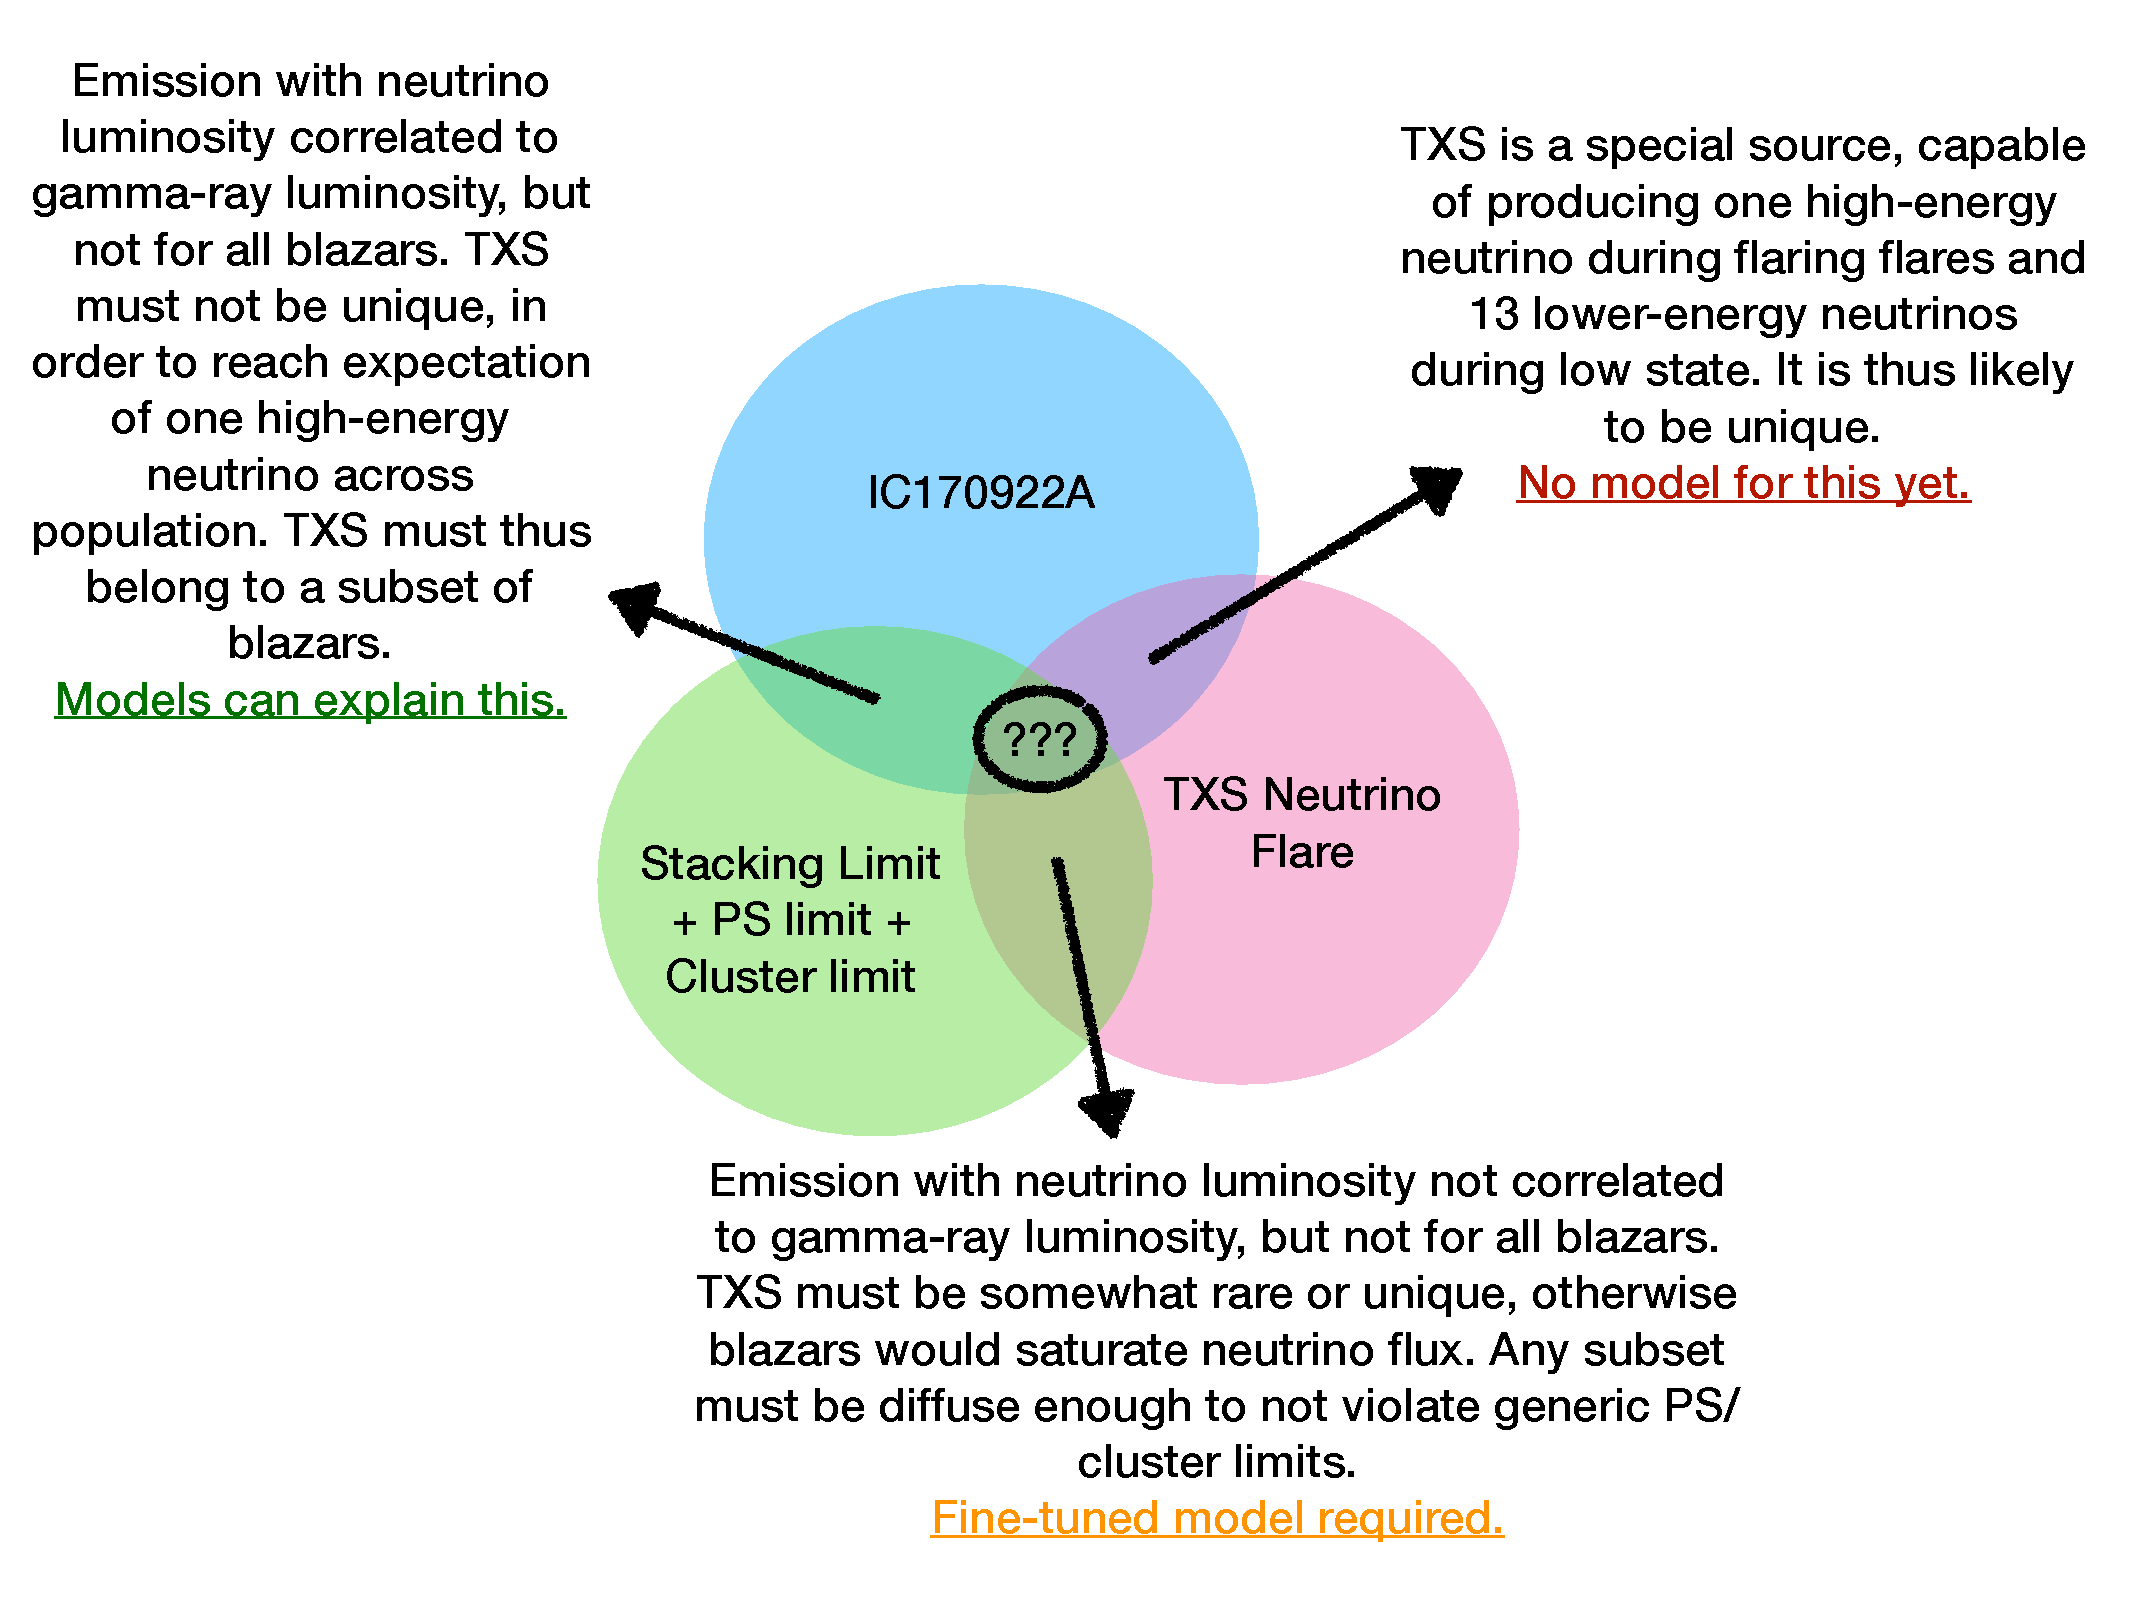
\includegraphics{txs_logic}
 	\caption{The challenge of coherently understanding the scenarios for neutrino emission from blazars, given the two pieces of evidence from TXS 0506+056, as well as the constraints from IceCube stacking analyses, general point-source searches and generic time-dependent cluster searches. To date, no model has resolved all three observations coherently.}
 	\label{fig:TXSLogic}
 \end{figure}
\section{Gamma-Ray Bursts}

Gamma-ray Bursts (GRBs) have long been proposed as a source of neutrinos. GRBs themselves fall into two broad categories, short and long, which are believed to arise from distinct physical populations. Long GRBs have been associated with the appearance of broad-lined type Ic supernova, and are thus believed to arise from a relativistic jet produced during supernova explosion. 

Short GRBs are now known to arise from relativistic jets launched during the merger of binary neutron stars. The first, and to date only, observed coincidence occurred for the gravitational wave event GW170817, which was associated with the short GRB 170817A and the kilonova AT2017gfo. Observations of GRB170817A revealed that it was particularly underluminous relative to most short GRBs, a fact later explained by comprehensive observations and modelling of AT2017gfo that confirmed an off-axis jet geometry. Given the relatively narrow jet opening angle, it is expected that the majority of future binary neutron star mergers detected by LIGO will not have detectable GRB counterparts.

Afterglow for both?

For both short and long GRBs, neutrino emission might be expected during the so-called "prompt phase" of gamma-ray emission. IceCube has undertaken numerous searches for neutrino emission, but has so far observed no correlation. Prompt emission from GRBs is particularly favourable for neutrino detection, because the brief and well-defined search period greatly reduces the expected background for such searches. This scenario is indeed one of the most-constrained by IceCube, which current limits restrict to less than 1\% of the astrophysical neutrino flux. 

Our understanding of GRBs has recently expanded further after the discovery of GRB VHE gamma-ray emission by MAGIC and HESS collaborations. The timescales for this emission, extending as much as 18 days after prompt phase indicates that high-energy processes extend throughout the so-called afterglow phase. consequently there is renewed focus on potential neutrino afterglow  emission, which is significantly less-constrained. One previous Icecube analysis limited the contribution to n\% (cite HESE).

An additional subclass are so-called low-luminosity GRBs (LLGRBs), believed to be... Given the poor efficiency with which source sources are detected, stacking searches of LLGRBs are significantly less powerful. However, for this case, generic searches for short-scale neutrino multiplets provide constraints on the contribution of such a population. In this case, they are known to contribute less than x\%.
\section{Core-Collapse Supernova}
 \begin{marginfigure}
	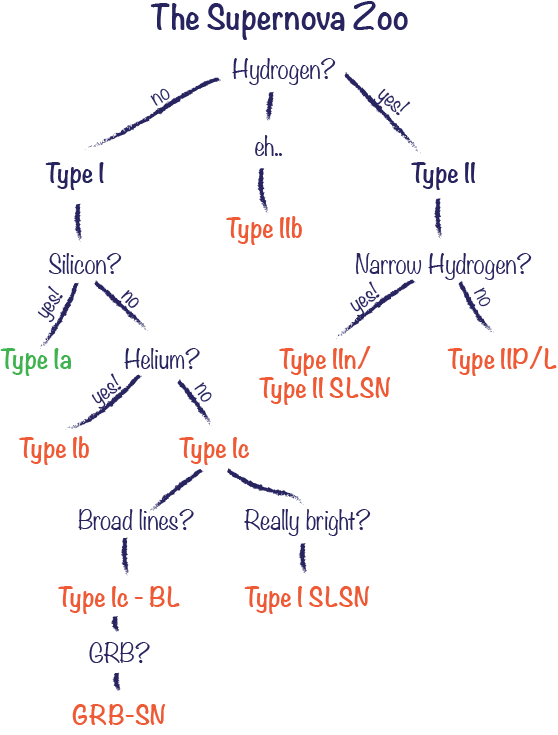
\includegraphics{sn_zoo-1}
	\caption{An overview of the current supernova classification scheme, which has been recently expanded to include superluminous supernova. Type 1a supernovae, marked in green, arise from thermonuclear explosions. All other classes, marked in origin, occur due to core collapse.}
	\labfig{fig:snzoo}
\end{marginfigure}
Supernovae, the explosive death of stars, are perhaps the best-studied phenomenon in astronomy. They are traditionally classified based on observed properties, rather than intrinsic physical attributes. An overview of a classification scheme is given in Figure \ref{fig:snzoo}. The most fundamental distinction is in explosion mechanism, with Type 1a SNe occuring due to thermonuclear explosions while all other classes are believed to arise from stellar core collapse. Further distinctions are made based on emission line, yielding the classes of Type Ib, Ic and Type II. Some SNe are observed to have narrow lines, which occur due to interaction with ejecta and circumstellar material (CSM). These supernova are denoted with 'n', the most common being Type IIn. This group in particular are candidate neutrino sources, in which neutrinos are produced via CSM interactions. An additional class of SNe is the IIP subclass, the subset of Type II SNe for which a characteristic lightcurve plateau is observed. Such plateaus are typically assumed to arise from....
Those Type II supernova not falling into IIp are instead classified as IIL, with characteristic Linear decay lighcurves.

Type Ic SNe can occasionally be observed with spectroscopic features known as Broad-Lines, which typically indicate the presence of fast-moving material. These form a distinct sublass, and it is this subclass which has been associated with long GRBs. Though radio observations have excluded the possibility that all Ic-BL SNe host relativistic jets? it is expected that even those without an observed GRB may instead host so-called 'choked jets' . These occur if a relativistic jet is lauched during core collapse, but because it lacks sufficient power to break through the outer layers of stellar material, it is stopped within the interior of the star. These choked jets, much like their standard counterparts, could produce neutrino emission. This scenario is however particularly difficult to test, because only those choked jets aligned towards Earth would produce a neutrino signal. As the alignment of a choked jet cannot be measured, it is impossible for us to say which supernova should or should not produce neutrinos. 

An additional category of supernovae has been recently observed, identifiable by their atypical brightness. So-called Superluminous supernovae (SLSNe) were initially classified as any SNe with an absolure magnitude brighter than -21 mag. However, in recent years, increased study has led to a spectroscopic classification being favoured, with some dimmer objects in the range $-20 < M < -21$ also being accepted. There are currently two favoured models to explain why SLSNe are so bright, namely the Magnetar model and the PISN model. .....

\section{Tidal Disruption Events (TDEs)}
== Roche Limit==
The tidal radius can best be understood by comparison to the more straightforward concept of the Roche Limit, otherwise known as the Roche Radius. The Roche Radius is defined as the distance at which the self-gravitiational force acting on the outer surface of a body are exactly equal to the gravitational pull of a second body on that same mass element. If a star moves closer than its Roche Radius for an SMBH, there will be a net force on mass elements on the star surface towards the SMBH, and the star will disintegrate.

The Tidal Force of one body acting on another is simply the difference in gravitational force strength between the closer surface of the sphere and its core. The Tidal Force of a black hole of mass M and distance d, acting on a mass element u lying on the closest point of the stellar surface, is thus given by:

$F_{tidal} = \frac{GMu}{(d-r)^{2}} - \frac{GMu}{(d)^{2}}$

$F_{tidal} = \frac{GMu}{d^{2}}((1-\frac{r}{d})^{-2} - 1 )$

Using Binomial Expansion with the reasonable assumption that r<<d, we reach an approximation:

$F_{tidal} \approx \frac{GMu}{d^{2}}\times \frac{2r}{d}$
The Roche Radius for a black hole of mass M for a star of mass m and radius r is thus found by equating this with the self-gravitational force acting on the same mass element. 

$F_{grav} = \frac{Gmu}{r^{2}} = \frac{2GMur}{d^{3}} \approx F_{tidal}$

$ d = r \times (\frac{2M}{m})^{\frac{1}{3}} \approx r_{roche}$

== Tidal Radius ==

This simplistic model does not hold for Tidal Disruption Events. The tidally-disrupted body would need to be in a circular orbit with synchronised spin, but stars tend to have approach Black Holes parabolically. In addition to Angular Momentum, General Relativity should be accounted for. This is particularly relevant for large black holes. A rigorous definition of Tidal radius should account for these things, but in any case, the point at which a star becomes 'tidally disrupted' is difficult to define. An event which only strips a fraction of the outer shell of the star would be ambiguous. Fortunately these definitions differ only by the order of unity from the Roche Radius. In the original paper introducing these calculations by [https://www.nature.com/nature/journal/v333/n6173/abs/333523a0.html Rees (1988)], the tidal radius was defined as the radius at which the mean internal density of the star is exceed by the mean internal density of the orbital volume. In this definition:

$\rho_{star} = \frac{m}{\frac{4}{3} \pi r ^{3}}  = \frac{M}{\frac{4}{3} \pi d ^{3}}= \rho_{volume}$

$ d = r \times (\frac{M}{m})^{\frac{1}{3}} = r_{tidal} $

Thus we see that:

$ r_{tidal} = \frac{r_{roche}}{\sqrt[3]{2}} $

In any definition of a characteristic tidal radius, we nonetheless always find that the radius scales with the cubic root of mass. It is interesting to recall that, in contrast, the Schwarzschild Radius of a black hole scales linearly with its mass. 

$R_{S} = \frac{2GM}{c^{2}}$

Consequently, the Schwarzschild Radius of the Black Hole grows faster as a function of Mass than the tidal radius. There is thus a critical black hole mass, for which the Schwarzschild Radius equals the star's Tidal Radius. Above this, a TDE cannot occur, because the star would have to be wholly swallowed by the black hole in order to be tidally disrupted. Though the exact limit will vary somewhat depending on the mass of the star, using typical values gives us an order-of-magnitude upper limit on TDE-generating black holes of $M < 10^{8} M_{\odot}$.

== Post-Disruption Evolution ==

For TDEs, the accretion of stellar material produces a highly-luminous flare, which is often the cause of discovery. This can be visible in Optical, UV or XRays. The bound mass spirals into the Black hole, but the fall-in time of each mass element in the bound material depends on the Gravitational Potential Energy of the element, leading to a characteristic fall-in rate $ \frac{dM}{dt} \propto t^{\frac{5}{3}}$ relation. This, in turn, can be seen in the light curves of TDEs.

There is evidence to support the existence of jetted TDEs, and these are usually highly-luminous in X rays. However, the classification of candidates into jetted or non-jetted can be unclear.

There is a further proposed model in which an envelope forms around the Black Hole, which could lead to choked jets.

== Neutrino Emission ==

The process for neutrino emission in TDEs, as well as the expected rates and neutrino light curves, are all highly uncertain. A key component of this analysis will be to probe the importance of an accurate time PDF, and the degree to which a minimal-assumption wide box model is the optimal time PDF to use. Even assuming the shape of the expected light curve was well known for each TDE (either the same neutrino light curve for every TDE,  or one closely correlated to the TDE optical or X Ray light curve), there remains a sigificant degree of uncertainty regarding the delay between neutrino emmision and optical emmission. It is possible that the peak neutrino emission is achieved more than 100 days before optical peak, but the expected gap is entirely model-dependent. The following potential models have been proposed for Neutrino Acceleration:

* Jetted TDEs, such as Swift J1644-57
* Choked Jet Scenario

Tidal Disruption Events (TDEs) are rare transients that occur when stars pass close to supermassive black holes (SMBHs). Studies have suggested that TDEs are sources of high-energy neutrinos and ultra-high energy cosmic rays\cite{2009ApJ...693..329F,2017MNRAS.469.1354D}, in particular those TDEs with relativistic particle jets\cite{2014arXiv1411.0704F,2017ApJ...838....3S,2016PhRvD..93h3005W,2017PhRvD..95l3001L}. TDEs with non-thermal radio emission are considered the most likely candidates for sources of high-energy neutrinos.

\section{Fast Radio Bursts}

A relatively recent astro

\section{Active Galactic Nuclei and Starburst Galaxies}
One additional possibility is that the astrophysical neutrino flux is produced by a large population of steady sources, and is thus truly a \textbf{diffuse} astrophysical neutrino flux. One case would be for neutrino production in Starburst Galaxies, which has been suggested in various models x.

Starburst galaxies are those galaxies for which there is a high level of star formation. Such galaxies have elevated supernovae rates, and are typically bright in UV and such. Starburst galaxies have been detected in gamma rays, including at very high energies, confirming the existence of acceleration processes. A search for neutrino emission from Starburst Galaxies was performed in x, and no significant correlation was identified. Given the expected dominant contribution from unresolved Starburst galaxies to any population neutrino flux, and accounting for the fact that this aggregate flux must not exceed the measured astrophysical neutrino flux, it is clear that the nearby starburst galaxies must therefore be very weak neutrino emitters. Such a scenario is unfavourable for identification against an isotropic neutrino background, and in this case it is unlikely that IceCube would have sufficient sensitivity to identify the neutrino flux origin.

A similar case would occur in that case of neutrino production from the cores of Active Galactic Nuclei (AGN), as suggested by XYZ. Here neutrinos would arise from pn interaction occurring in the inner accretion disk of AGN, with the corresponding gamma-ray emission being absorbed. Such a scenario is appealing theoretically, as it would neatly evade the existing constraints on diffuse gamma-ray emission, which we know to arise predominantly from blazars. This hypothesis was tested by IceCube (I hope...)

SUMMARY TABLE with source class, limit, and spectral index
\setchapterimage[6.5cm]{Grid_FullView_Logo}
\setchapterpreamble[u]{\margintoc}
\chapter{Realtime Multi-Messenger Astronomy}
\labch{realtime}
\begin{fquote}[Isaac Asimov][Lady Windermere's Fan][18??] A stopped clock is right twice a day.
\end{fquote}

In recent years, there has been a significant renewed interest in the study of transient and variable objects in astronomy. Driven primarily by the speed at which objects can evolve and disappear, particularly GRBs and latterly Kilonovae, it is often essential that astronomy can be done with minimal latency. In this vein, it is now commonplace for detectors to automatically issue so-called alerts for observations that meet given criteria, to enable other instruments to rapidly obtain near-simultaneous observations. Realtime alerts are automatically issued by GRB-searching instruments such as Swift-BAT and Fermi-GBM, while gravitaional-wave events are issued by the LIGO-VIRGO observatories, and high-energy neutrino alerts are issued by IceCube as well as ANTARES.

These alerts are all typically issued via  the Gamma-ray Coordination Network (GCN) system, where observatories can subscribe to automatically be notified or point.  An essential component of this process is the additional information published by astronomers, via GCN or Astronomers Telegrams (ATELs), in which follow-up observations are coordinated. There have been two high-profile examples of this, namely the comprehensive followup of GW170817/GRB170817A that led to the first unambiguous observation of a kilonovae, and the followup of high-energy neutrino IC170922A, which led to the identification of TXS 0506+056 as the first candidate source of TeV neutrinos. 

As part of this thesis, the author maintained and further developed the IceCube Realtime System from October 2018 onwards, acting as first responder to the vast majority of neutrino alerts in that period.

\section{The IceCube Realtime System}
The IceCube Realtime System has been operating since 2016, providing the first source of high-energy neutrino alerts. The first iteration of the alert system consisted of two streams, namely High-Energy Starting Events (HESE) and Extremely High Energy (EHE) events CITE. Each was an established event selection used to identify likely-astrophysical neutrinos cite. Filters to identify relevant events are deployed on computers at the South Pole, and detections are flagged  with low latency. After fast "online" reconstruction algorithms are applied to events, an automated machine-readable "notice" is distributed via the GCN system. In parallel, data from the event is transmitted via satellite to a computing centre in Madison, Wisconsin where a full likelihood scan is performed on the event (see chapter \ref{ch:Event Selection and Reconstruction} for more details). 

Give V1 rates!

The alerts are vetted by humans to asses the event quality, with visually inspection being used to confirm classified topology and event reconstructions. The operating state of the detector is additionally checked. Following these steps, a plain-text GCN circular is distrubuted via the GCN system to confirm the good nature of the alert, and to provide the updated localisation arising from the full scan. 

This original system of alerts continued until May 2019, at which point a new alert system was implemented. While the original EHE selection was maintained, the HESE alert selection was improved to reduce the cascade contamination, and improve the astrophysical purity. In addition, a new alert stream based on the GFU event selection was initiated, with a significantly-elevated rate relative to EHE and HESE alerts. The publication of these three alert streams was unified into a new IceCube Astrotrack GCN stream, which was further subdivided into Gold and Bronze based on the average purity of alerts. Golden Astrotrack alerts will, as an ensemble, have an average of 50\% astrophysical neutrinos, while Bronze Astrotrack will have an average of 30\% astrophysical neutrinos.

A summary of all neutrino alerts issued to date is provided in table X. Individual neutrino alerts of interest are summarised in subsequent sections. 

\subsection{IC160427A - The "PanSTARRS Supernova Neutrino"}

The first alert issued under this system, HESE alert IC160427A, was found to be in spatial coincidence with an optical transient detected by the Pan-STARRS Observatory while following up the alert. This transient was initially tentaively classified as a Type Ic supernova, for which various models have predicted neutrino emission (see Chapter \ref{ch:sources}).  However, the further spectroscopic and photometric evolution indicated that this was  more likely a Type Ia Supernova, for which no neutrino emission would be expected. Nonetheless, dedicated efforts to simulate an ensemble of IC160427A-like events led to the first characterisation of the impact of systematic uncertainties in modelling the polar glacial ice on directional reconstruction with IceCube for high-energy alerts. 

\subsection{IC170922A The "TXS 0506+056 Neutrino"}
Subsequent neutrino alerts did not yield any probable counterparts, until the detection of EHE alert IC170922A in spatial coincidence with flaring blazar TXS 0506+056. Chance coincidence in this case was estimated  This event was also resimulated in the same manner as IC160427A. Remarkably, despite its radically-different topology of through-going muon rather than starting track, the results were found to be broadly consistent. More details are given in chapter N.

\subsection{IC190331A - The "Multi-PEV Neutrino"}

A starting track was observed 

\subsection{IC190730A - The "ICRC Neutrino"}

IC190730A was a golden neutrino alert with a signalness of roughly 65\%. Following the automated notice, Millipede Reconstruction clearly showed it was well-localised, and spatially coincident with blazar PKS 1502+106. This particular blazar is extremely bright, being Nth brightest in the sky in terms of integrated gamma-ray energy flux, and owing to its high redshift of z=1.84, is one of the most luminous known blazars. This coincidence was reported in the corresponding GCN circular, and triggered a broad multi-wavelength follow-up campaign. The archival SED is provided in figure N, originally from X, but annotated to illustrate contemporaneous observations from other instruments.

\begin{figure}[!ht]
	\centering 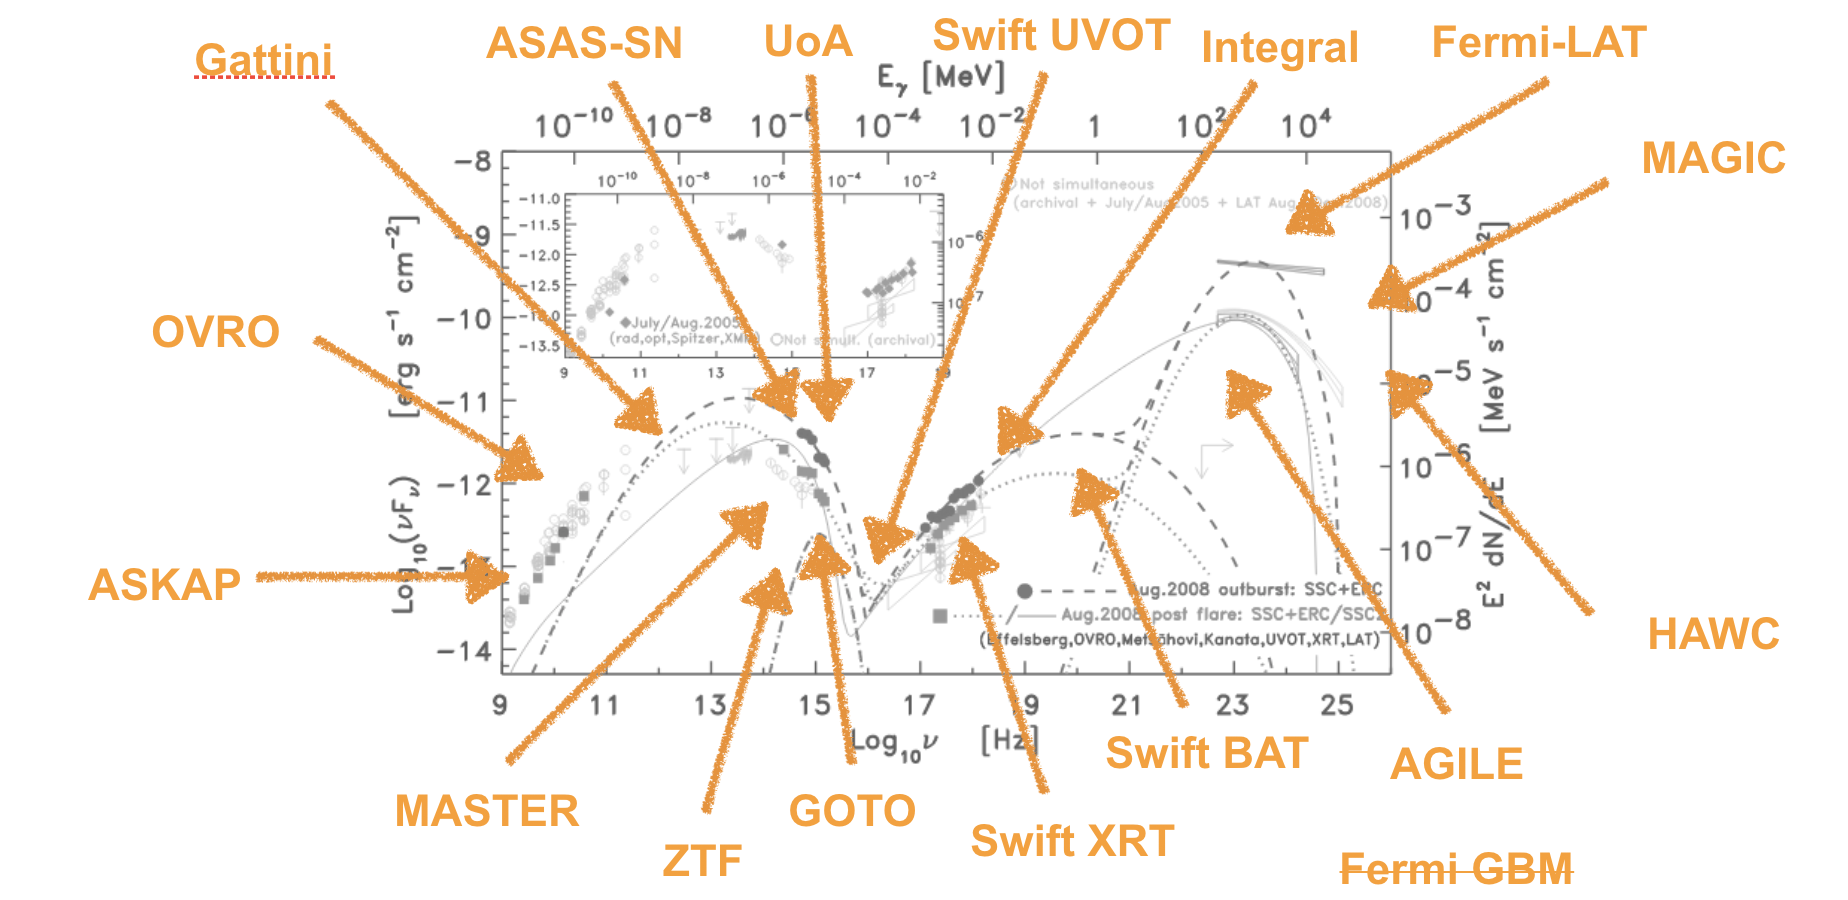
\includegraphics{pks_followup}
	\caption{The archival SED of PKS 1502+106 from X is shown. In orange, the names of various instruments that observed the source are overlaid, with orange arrows to indicate their corresponding energy regimes. CITEA-Z}
	\label{fig:PKSobs}
\end{figure}

Despite comprehensive wavelength coverage, 

The chance coincidence for at least one neutrino alert to be coincident with any of the  15 brightest blazars was calculated by the author, and found to be disfavoured at the level of 2.n sigma following the procedure in N. 

\subsection{IC190922B - The "SN2019pqh Neutrino"}

\subsection{IC191001A - The "Bran Stark Neutrino"}

\subsection{IC200107A - The "Flaring Extreme Blazar neutrino"}

\section{Interpreting high-energy neutrino alerts}

lalala

\subsection{Cluster searches}
lalaland

\subsection{OFU and GFU}.
\setchapterpreamble[u]{\margintoc}
\chapter{Overflow}
\labch{options}
\begin{fquote}[Henri Poincare][Lady Windermere's Fan][18??] Without interpolation all science would be impossible. 
\end{fquote}
\begin{fquote}[Feynman][Lady Windermere's Fan][18??] In theory there is no difference between theory and practice. In practise, there is.
\end{fquote}
\begin{fquote}[Douglas Adams][The Hitchiker's Guide to the Galaxy][18??] A neutrino is not a big thing to be hit by. In fact it's hard to think of anything much smaller by which one could reasonably hope to be hit. And it's not as if being hit by neutrinos was in itself a particularly unusual event for something the size of the Earth. Far from it. It would be an unusual nanosecond in which the Earth was not hit by several billion passing neutrinos.
\end{fquote}
\section{The Zwicky Transient Facility (ZTF)}
\begin{fquote}[Oscar Wilde][Lady Windermere's Fan][18??]We are all in the gutter, but some of us are looking at the stars
\end{fquote}

\section{Event Selection}

\subsection{Event Reconstruction}
\subsection{Angular Errors}

ns bias as function of ...

\section{Diffuse Astrophysical Neutrino Flux}

\section{Neutrinos from Optical Transients}
\subsection{The Plot}
sensitivity versus depth
Alerts vs ZTF

Cosmology + The PLOT

Eddington Bias?

As far back as X, when nuclear fusion was proposed as a mechanism to power the sun, it was expected that a flux of solar neutrinos should be detectable on Earth. This prediction was confirmed by early neutrino detectors, ZZ and Z, which measured the flux xyc.
The discovery of a source of neutrinos from beyond the solar system followed soon after, with the detection of nearby supernova SN1987A. Nearby supernova occur either within our galaxy, or in the neighbouring Magellanic clouds, at a rate of a couple per century. In thie case of SN1987A, the detection of the supernova was preceded by simultaneous detections of an elevated neutrino flux in multiple detectors on Earth. The coincident detection of photons and neutrinos marjked the first multi-messenger detection of an astrophysical source.

It is now well-understood that there is a diffuse flux of MeV-neutrinos produced from SN?, and preparations are underway for the inevitable next nearby SN, coordinated by the SuperNova Early Warning System (SNEWS). Given the increased volume of current-generation neutrino detectors, the next nearby supernova will be measured with much greater precision. IceCube itself will contribute to this, through a dedicated supernova detection system. Given the detector geometry, IceCube will not be able to identify individual neutrino events, nor reconstruct their directions. However, an increase in DOM noise will be clearly measurable, and likely with sufficiently resolution to resolve the time-evolution of the signal. 

In both cases, the neutrinos detected at MeV-energies.  However, in light of the discovery of a flux of high-energy astrophysical neutrinos by IceCube, a new branch of astronomy has developed searching for sources of these astrophysical neutrinos. The central fact for neutrino astronomy, at least in the ~TeV-PeV range for which IceCube is sensitive, is that at lower energies there is an overwhelming background, while at higher energies, statistics are poor. This is illustrated in Fig. The power of IceCube to detect an astrophysical flux depends on the degree to which this differs from the atmospheric background. Above all, the expected energy distribution for most astrophysical sources likely differs from the soft-spectrum atmospheric neutrino flux. In addition, the spatial distribution of the background is broadly isotropic, and uniform as a function of right ascension. The temporal distribution of this background, beyond small-scale season variations, is also reasonably isotropic. Foreground fuxes which differ substantially will be most easily detected.

The expected degree of anisotropy in the extragalactic astrophysical neutrino flux strongly depends on the properties of the assumed sources, in particular their density and source evolution. The source evolution describes the rate or density evolution of astrophysical objects as a function of redshift. For sources with a negative source evolution, the density in the local universe is greater than at high redshift, so there are fewer neutrinos produced by distant, unresolved sources. Conversely, for a strongly positive source evolution, we expect a greater fraction of neutrinos to arrive from unresolved sources. When local density and source evolution are coupled, we then find arrive at a flux which anisotropic to varying degrees. Given that the atmospheric backgrounds are broadly isotropic, and uniform as a function of right ascension, the sensitivity of IceCube to a given astrophysical flux will depend strongly on whether that flux is sufficiently spatially anistotropic to distinguish it from atmospheric backgrounds. A higher-density source population, with positive evolution, would be much harder to identify that a low-density one with negative evolution. Anisotropy in neutrino arrival times can be an additional metric to distinguish astrophysical neutrinos. For sources which are variable or transient, neutrino emission is only expected for distinct time periods, eliminating background events.

In general, given knowledge about the background, the most agnostic methods to identify neutrino sources look for clustering within the data without reference to external datasets. Such auto-correlation analyses can be done with either a time-integrated or time-dependent all-sky likelihood scan. The result of such an analysis is a pixelised likelihood map. Comparisons of this map can then be made to expectations from background, either using the single "hottest spot" in the sky, or by comparing the distribution of hotspots. No significant excess was found for either approach, providing significant general constraints on neutrino source populations, . Given the current detector volumes and resolution, as well as the lack of observed lower-significance overfluctuations, it appears that the astrophysical neutrino flux is not sufficiently anisotropic for auto-correlation analyses to discover a neutrino source in the near future.

As an alternative to agnostic searches, specific source hypothesis tests can be substantially more sensitive. Given the position of a known astrophysical object, the threshold for a significant excess is greatly reduced due to the avoidance of an all-sky trial factor. Sensitivity can be further enhanced when information from multiple objects is combined in a so-called 'stacking search'. These methods can be used to test for neutrino excesses correlated to astrophysical populations. One drawback of these methods is that their sensitivity strongly depends on the quality of available multi-wavelength data. Often these catalogues are not complete, particularly in the case of transient or variable objects. 

On the other hand, realtime analysis is a complementary method that inverts this traditional object neutrino relationship. Instead of taking a known object, and asking whether neutrinos are correlated to it, realtime analysis identifies likely-astrophysical neutrinos and seeks to identify coincident astrophysical objects that could potentially have produced the neutrino. The power of realtime searches is that they can, if a possible counterpart is identified, lead to contemporaneous multi-wavelength follow-up that maybe reveal more about a given object. Within this context, the 

However, it should be noted that both realtime and stacking analyses are only sensitive to cases where neutrino sources have detectable EM counterparts. It might however be the case that EM emission from neutrino sources is either absorbed or attenuated, and consequently stacking analyses will be unable to identify such EM-dark neutrino sources. Furthermore, particularly for CCSNe-like populations following the Star Formation Rate (SFR), a large fraction of the astrophysical neutrino might in fact come from unresolved sources.

Neutrino Astronomy with IceCube is rather distinct from more mature branches of astronomy, because we have much less power to distinguish astrophysical signal from background. This regime is to some extent fixed by the raw event rate, in which irreducible atmospheric backgrounds are overwhelmingly dominant over astrophysical neutrinos except at the highest energies. However, it is exacerbated by the limited angular resolution of the detector, where each IceCube event covers a relatively-large area of the sky. Further, owing to the limited effective area of IceCube, there are insufficient numbers of signal-like neutrinos to form cleanly-identifiable clusters. Fundamentally, there is almost no signature in data for which a background origin can be discounted.

It is thus not difficult to find interesting things that are correlated with neutrino arrival directions or times, such as weekends or star signs, because any individual hypothesis will have a small probability to be correlated with  neutrinos by chance. The sum of these many small probabilities can become a large probability, and unless we are careful to correct for this look-elsewhere effect, many spurious correlations will be found. To shield against this, anisotropies in neutrino data are studied through \emph{blind analysis}, in which methods are first developed using simulated datasets. Once an analysis method and hypothesis has been finalised, and the procedure for determining the significance of a result has been fixed, the analysis can then be repeated on real data.

\appendix % From here onwards, chapters are numbered with letters, as is the appendix convention

\pagelayout{wide} % No margins
\addpart{Appendix}
\pagelayout{margin} % Restore margins

\setchapterstyle{lines}
\labpage{appendix}
\blinddocument


%----------------------------------------------------------------------------------------

\backmatter % Denotes the end of the main document content

\setchapterstyle{plain} % Output plain chapters from this point onwards

%----------------------------------------------------------------------------------------
%	BIBLIOGRAPHY
%----------------------------------------------------------------------------------------

% The bibliography needs to be compiled with biber using your LaTeX editor, or on the command line with 'biber main' from the template directory

\defbibnote{bibnote}{Here are the references in citation order.\par\bigskip} % Prepend this text to the bibliography
\printbibliography[heading=bibintoc, title=Bibliography, prenote=bibnote] % Add the bibliography heading to the ToC, set the title of the bibliography and output the bibliography note

%----------------------------------------------------------------------------------------
%	NOMENCLATURE
%----------------------------------------------------------------------------------------

% The nomenclature needs to be compiled on the command line with 'makeindex main.nlo -s nomencl.ist -o main.nls' from the template directory

\nomenclature{$c$}{Speed of light in a vacuum inertial frame}
\nomenclature{$h$}{Planck constant}

\renewcommand{\nomname}{Notation} % Rename the default 'Nomenclature'
\renewcommand{\nompreamble}{The next list describes several symbols that will be later used within the body of the document.} % Prepend this text to the nomenclature

\printnomenclature % Output the nomenclature

%----------------------------------------------------------------------------------------
%	GREEK ALPHABET
% 	Originally from https://gitlab.com/jim.hefferon/linear-algebra
%----------------------------------------------------------------------------------------

\vspace{1cm}

{\usekomafont{chapter}Greek Letters with Pronounciation} \\[2ex]
\begin{center}
	\newcommand{\pronounced}[1]{\hspace*{.2em}\small\textit{#1}}
	\begin{tabular}{l l @{\hspace*{3em}} l l}
		\toprule
		Character & Name & Character & Name \\ 
		\midrule
		$\alpha$ & alpha \pronounced{AL-fuh} & $\nu$ & nu \pronounced{NEW} \\
		$\beta$ & beta \pronounced{BAY-tuh} & $\xi$, $\Xi$ & xi \pronounced{KSIGH} \\ 
		$\gamma$, $\Gamma$ & gamma \pronounced{GAM-muh} & o & omicron \pronounced{OM-uh-CRON} \\
		$\delta$, $\Delta$ & delta \pronounced{DEL-tuh} & $\pi$, $\Pi$ & pi \pronounced{PIE} \\
		$\epsilon$ & epsilon \pronounced{EP-suh-lon} & $\rho$ & rho \pronounced{ROW} \\
		$\zeta$ & zeta \pronounced{ZAY-tuh} & $\sigma$, $\Sigma$ & sigma \pronounced{SIG-muh} \\
		$\eta$ & eta \pronounced{AY-tuh} & $\tau$ & tau \pronounced{TOW (as in cow)} \\
		$\theta$, $\Theta$ & theta \pronounced{THAY-tuh} & $\upsilon$, $\Upsilon$ & upsilon \pronounced{OOP-suh-LON} \\
		$\iota$ & iota \pronounced{eye-OH-tuh} & $\phi$, $\Phi$ & phi \pronounced{FEE, or FI (as in hi)} \\
		$\kappa$ & kappa \pronounced{KAP-uh} & $\chi$ & chi \pronounced{KI (as in hi)} \\
		$\lambda$, $\Lambda$ & lambda \pronounced{LAM-duh} & $\psi$, $\Psi$ & psi \pronounced{SIGH, or PSIGH} \\
		$\mu$ & mu \pronounced{MEW} & $\omega$, $\Omega$ & omega \pronounced{oh-MAY-guh} \\
		\bottomrule
	\end{tabular} \\[1.5ex]
	Capitals shown are the ones that differ from Roman capitals.
\end{center}

%----------------------------------------------------------------------------------------
%	GLOSSARY
%----------------------------------------------------------------------------------------

% The glossary needs to be compiled on the command line with 'makeglossaries main' from the template directory

\newglossaryentry{computer}{
	name=computer,
	description={is a programmable machine that receives input, stores and manipulates data, and provides output in a useful format}
}

% Glossary entries (used in text with e.g. \acrfull{fpsLabel} or \acrshort{fpsLabel})
\newacronym[longplural={Frames per Second}]{fpsLabel}{FPS}{Frame per Second}
\newacronym[longplural={Tables of Contents}]{tocLabel}{TOC}{Table of Contents}

\setglossarystyle{listgroup} % Set the style of the glossary (see https://en.wikibooks.org/wiki/LaTeX/Glossary for a reference)
\printglossary[title=Special Terms, toctitle=List of Terms] % Output the glossary, 'title' is the chapter heading for the glossary, toctitle is the table of contents heading

%----------------------------------------------------------------------------------------
%	INDEX
%----------------------------------------------------------------------------------------

% The index needs to be compiled on the command line with 'makeindex main' from the template directory

\printindex % Output the index

%----------------------------------------------------------------------------------------
%	BACK COVER
%----------------------------------------------------------------------------------------

% If you have a PDF/image file that you want to use as a back cover, uncomment the following lines

%\clearpage
%\thispagestyle{empty}
%\null%
%\clearpage
%\includepdf{cover-back.pdf}

%----------------------------------------------------------------------------------------

\end{document}
